\documentclass{article}

% NeurIPS 2026 template — using main track (double-blind) for submission
\usepackage{neurips_2026}
% After acceptance, use: \usepackage[main, final]{neurips_2026}
% For E&D track: \usepackage[eandd]{neurips_2026}

\usepackage[utf8]{inputenc}
\usepackage[T1]{fontenc}
\usepackage{hyperref}
\usepackage{url}
\usepackage{booktabs}
\usepackage{amsfonts}
\usepackage{amsmath}
\usepackage{amssymb}
\usepackage{nicefrac}
\usepackage{microtype}
\usepackage{xcolor}
\usepackage{graphicx}
\usepackage{multirow}
\usepackage{subcaption}
\usepackage{algorithm}
\usepackage{algorithmic}
\usepackage{tikz}
\usetikzlibrary{shapes,arrows,positioning,fit,calc}
\usepackage{wrapfig}
\usepackage{enumitem}
\usepackage{pifont}
\usepackage{colortbl}

% --- Custom commands ---
\newcommand{\gym}{\textsc{Healthcare AI GYM}}
\newcommand{\ours}{\textsc{GYM-RL}}
\newcommand{\todo}[1]{\textcolor{red}{\textbf{[TODO: #1]}}}
\newcommand{\rq}[1]{\textbf{RQ#1}}

\title{\gym{}: A Unified Gymnasium for Training and Analyzing \\
Generalizable Medical AI Agents across Modalities}

\author{%
  Minbyul Jeong \\
  % Affiliation \\
  % \texttt{email} \\
}

\begin{document}

\maketitle

% ============================================================
\begin{abstract}
% ============================================================
Can a single training environment produce medical AI agents that generalize across text QA, visual diagnosis, and EHR reasoning? We present \gym{}, a Gymnasium-compatible environment spanning 10 clinical domains with 195K+ tasks and 187+ tools, designed as a unified playground for training and analyzing medical AI with reinforcement learning. Through controlled experiments on Lingshu-7B with SFT warmup followed by four GRPO-family RL algorithms, we find: (1) \textbf{Sub-epoch phase transition with peak convergence but stability divergence}: SFT provides initial gains (MedQA 9\%$\to$39\%), then RL produces a phase transition after just 0.25 epochs (39\%$\to$57\%). All four algorithms converge to within 0.4~pp at their peak, but diverge in stability: GRPO sustains performance for 1.25 epochs while Dr.~GRPO collapses after 0.875 epochs---revealing that \textbf{algorithmic simplicity, not sophistication, drives robustness}. (2) \textbf{Cross-modal transfer decomposes into two mechanisms}: format compliance from SFT (PMC-VQA 0.2\%$\to$37.7\%; RL adds nothing) and fragile knowledge transfer from RL (SLAKE +2.1~pp beyond SFT at step 100, $p{=}0.023$; vanishes by step 150). (3) \textbf{RL is task-type selective}: it adds no value for long-form generation (5 benchmarks) or agentic EHR reasoning (MIMIC-III: $\pm$0.6~pp of SFT-only). (4) \textbf{Narrow optimal training window with catastrophic forgetting}: a transient dip at 0.75 epochs fully recovers for individual algorithms, but performance collapses to 30\% MedQA (below SFT-only) by epoch 2---revealing that medical RL overtraining is dangerous. The GSPO+DAPO combination's equivalent dip is \emph{permanent}, motivating single-algorithm training with dense checkpoint evaluation. (5) \textbf{On-policy distillation (OPD) stabilizes training beyond the forgetting boundary}: cross-stage OPD with an SFT teacher and RL student sustains 10 epochs without catastrophic forgetting. The blending coefficient $\alpha$ controls qualitative KL regime transitions: $\alpha{=}0.5$ produces monotonic KL growth (plateau ${\sim}7$), while $\alpha{=}0.3$ produces bounded oscillation ($[1.8, 2.6]$)---with identical downstream performance, making $\alpha{=}0.3$ strictly Pareto-dominant. We release our environment and evaluation suite for reproducible medical AI research.
\end{abstract}

% ============================================================
\section{Introduction}
\label{sec:intro}
% ============================================================

\subsection{Why Healthcare AI Needs a Gymnasium}

Medical AI has achieved impressive results on individual benchmarks. GPT-4 surpasses the USMLE passing threshold on MedQA~\citep{nori2023gpt4}. Med-PaLM 2 approaches expert-level performance on medical question answering~\citep{singhal2023medpalm2}. Specialized vision-language models achieve strong results on radiology VQA~\citep{chen2024huatuogpt}. Yet a fundamental problem persists: \textbf{no single model excels across the full spectrum of clinical tasks.}

Consider what a competent medical AI system must actually do:
\begin{itemize}[nosep, leftmargin=*]
    \item \textbf{Text-based reasoning}: Answer USMLE-style questions requiring multi-step clinical logic (MedQA, MedMCQA, MMLU-Medical).
    \item \textbf{Visual diagnosis}: Interpret radiology images, pathology slides, and clinical photographs (VQA-RAD, PathVQA, SLAKE).
    \item \textbf{EHR comprehension}: Navigate electronic health records, track lab trends, compute clinical scores, and make disposition decisions (MIMIC-III, eICU).
    \item \textbf{Safety-critical reasoning}: Avoid prescribing contraindicated drugs, recognize emergencies, and flag uncertainty.
\end{itemize}

These capabilities are currently developed and evaluated in \emph{complete isolation}. A model fine-tuned for MedQA is never tested on VQA-RAD. A radiology VQA model cannot navigate an EHR. There is no shared training environment where these skills are learned together, and no systematic way to compare whether RL algorithm A produces more generalizable medical reasoning than algorithm B across model families.

\subsection{The Missing Infrastructure}

This fragmentation stems from a missing piece of infrastructure. In robotics, standardized environments like Gymnasium~\citep{towers2024gymnasium} and MuJoCo have enabled systematic comparison of RL algorithms across tasks, leading to rapid methodological progress. In medical AI, no such infrastructure exists. Researchers are left to:

\begin{enumerate}[nosep, leftmargin=*]
    \item Build custom training pipelines for each benchmark, making cross-benchmark comparison difficult.
    \item Evaluate on a single modality (text OR vision OR EHR), missing the full picture of medical competence.
    \item Report results on one model architecture, with no evidence that findings transfer to other model families.
    \item Use ad-hoc reward functions, making it impossible to attribute improvements to the RL algorithm vs.\ the reward design.
\end{enumerate}

Recent work has begun to address this. MedAgentGym~\citep{medagentgym2026} provides a Gymnasium interface for medical agents, and AgentClinic~\citep{schmidgall2025agentclinic} simulates clinical encounters. However, these cover only text-based medical QA and clinical diagnosis respectively, leaving vision and EHR tasks unaddressed. More critically, they do not provide the systematic experimental framework needed to compare RL strategies across model families.

\subsection{Our Approach: A Playground for Medical AI}

We introduce \gym{}, designed around a simple principle: \textbf{bring any model into the gymnasium, train it with any RL algorithm, and measure what it learns across all modalities.}

The gymnasium spans 10 clinical domains with unified tool interfaces, a shared knowledge base of 828K medical passages, and a 5-dimensional reward system that evaluates not just accuracy but also clinical process, safety, format, and coherence. Critically, every experiment we conduct follows a disciplined protocol:

\begin{enumerate}[nosep, leftmargin=*]
    \item \textbf{Motivation}: Why is this experiment necessary? What gap does it address?
    \item \textbf{Hypothesis}: What specific, falsifiable prediction do we test?
    \item \textbf{Validation}: How do we test this prediction with proper controls and statistical rigor?
    \item \textbf{Generalization}: Does the finding hold across different model families and domains?
\end{enumerate}

This discipline transforms medical AI training from an ad-hoc fine-tuning exercise into a systematic scientific investigation.

Table~\ref{tab:comparison} positions \gym{} relative to existing medical AI environments.

\begin{table}[t]
\centering
\caption{Comparison with existing medical AI training approaches. We separate training \emph{environments} (with interactive tool use and Gym API) from \emph{RL training methods} (applied to static datasets). Domain counts reflect distinct clinical task categories.}
\label{tab:comparison}
\resizebox{\textwidth}{!}{
\begin{tabular}{llccccc}
\toprule
\textbf{Type} & \textbf{System} & \textbf{Domains} & \textbf{Modalities} & \textbf{Tools} & \textbf{Safety Reward} & \textbf{RL Comparison} \\
\midrule
\multirow{3}{*}{Environment}
& AgentClinic~\citep{schmidgall2025agentclinic} & 1 (diagnosis) & Text & \ding{51}\textsuperscript{a} & \ding{55} & \ding{55} \\
& MedAgentGym~\citep{medagentgym2026} & 2 (QA, clinical) & Text & \ding{51} & \ding{55} & \ding{55} \\
& \textbf{\gym{} (Ours)} & \textbf{10} & \textbf{Text+Vision+EHR} & \textbf{\ding{51}} & \textbf{\ding{51}} & \textbf{\ding{51}} \\
\midrule
\multirow{3}{*}{RL Method}
& Med-R1~\citep{lai2025medr1} & 1 (radiology) & Vision & \ding{55} & \ding{55} & \ding{55} \\
& MedVLM-R1~\citep{pan2025medvlmr1} & 1 (radiology) & Vision & \ding{55} & \ding{55} & \ding{55} \\
& MediX-R1~\citep{medixr1} & 1 (radiology) & Vision & \ding{55} & \ding{55} & \ding{55} \\
\bottomrule
\multicolumn{7}{l}{\textsuperscript{a}\footnotesize AgentClinic supports simulated clinical interactions (ordering tests, interpreting results) but not multi-domain tool registries.} \\
\end{tabular}
}
\end{table}

\subsection{Contributions}

\begin{enumerate}[leftmargin=*]
    \item \textbf{Multi-Modal Medical Gymnasium} (\S\ref{sec:environment}): A comprehensive medical AI training and evaluation environment spanning text QA, visual diagnosis, EHR reasoning, and 7 additional clinical domains under a single Gymnasium API, with tool-use scaffolding for agentic training.

    \item \textbf{Empirical Analysis of SFT$\to$RL Training Dynamics} (\S\ref{sec:results}): Through controlled experiments on Lingshu-7B with SFT warmup followed by GRPO-family RL, we characterize four key phenomena: (a) SFT as the dominant driver of initial improvement (MedQA 9\%$\to$39\%); (b) RL producing a sub-epoch phase transition at 0.25 epochs ($+18$ pp MedQA, sustained through 1.25 epochs with transient oscillation at 0.75 epochs and recovery, but catastrophic forgetting by epoch 2); (c) RL adding no value for long-form generation; (d) EHR agentic task performance remaining modality-orthogonal to text RL.

    \item \textbf{Cross-Modal Transfer Decomposition} (\S\ref{sec:results}): Evidence that text-only training transfers to vision QA through two distinct mechanisms with different origins: format compliance from SFT (PMC-VQA: 0.2\%$\to$37.7\%, RL adds nothing) and knowledge transfer (SLAKE: $+3.8$ pp total vs.\ base at RL100, $p{=}0.023$; of which $+2.1$ pp is RL-specific beyond SFT), but the knowledge component is fragile---decays by RL150.

    \item \textbf{Sub-Epoch Phase Transition \& Catastrophic Forgetting} (\S\ref{sec:analysis}): Discovery that all four GRPO-family algorithms independently undergo an identical phase transition at just 0.25 epochs (${\sim}18$ pp MedQA jump)---after seeing only 25\% of training data---sustained through 1.25 epochs with a transient dip at 0.75 epochs that recovers by 0.875 epochs. However, by epoch 2, performance collapses below SFT-only (30\% MedQA), revealing a narrow optimal training window. The GSPO+DAPO combination shows the same dip but \textbf{fails to recover}, motivating single-algorithm training with early stopping.

    \item \textbf{Cross-Stage On-Policy Distillation with $\alpha$-Controlled KL Regimes} (\S\ref{sec:opd}, \S\ref{sec:opd_results}): We introduce cross-stage OPD that blends SFT teacher advantages with RL advantages via a per-token $\alpha$-weighted formulation. Through controlled $\alpha$ ablation, we discover that $\alpha$ acts as a KL regime control knob: $\alpha{=}0.5$ produces monotonic KL growth while $\alpha{=}0.3$ produces bounded oscillation---a qualitative regime change from a quantitative parameter shift, with identical downstream performance. This is the first OPD application in medical AI and the first analysis of $\alpha$--KL regime dynamics in any domain.

    \item \textbf{Evaluation Infrastructure} (\S\ref{sec:experiments}): Standardized evaluation across 21 benchmarks, 3 model architectures, and 4 task categories, with infrastructure for systematic RL algorithm comparison and reward ablation.
\end{enumerate}


% ============================================================
\section{Related Work}
\label{sec:related}
% ============================================================

\paragraph{Medical LLMs and VLMs.}
Medical question answering has been extensively studied through benchmarks such as MedQA~\citep{jin2021medqa}, MedMCQA~\citep{pal2022medmcqa}, and PubMedQA~\citep{jin2019pubmedqa}. Large models including GPT-4~\citep{nori2023gpt4}, Med-PaLM 2~\citep{singhal2023medpalm2}, and HuatuoGPT-o1~\citep{chen2024huatuogpt} have achieved strong results on text QA. For visual medical understanding, LLaVA-Med~\citep{li2023llavamed}, BiomedGPT~\citep{zhang2024biomedgpt}, and Med-PaLM M~\citep{tu2024medpalmm} have been developed. Med-PaLM M demonstrated positive cross-task transfer in joint multimodal training, and BiomedGPT achieved 16 SOTA results across 26 datasets. However, \textbf{no existing work trains and evaluates models across text QA, visual diagnosis, AND EHR reasoning within a single RL environment}---each community operates in isolation.

\paragraph{Medical AI Agents.}
AgentClinic~\citep{schmidgall2025agentclinic} simulates patient-doctor interactions for diagnostic reasoning. MedAgentGym~\citep{medagentgym2026} provides a Gymnasium interface for training medical agents with RL, achieving +42.47\% improvement via SFT warmup followed by RL. These represent important steps but cover only 1--2 domains and do not support visual or EHR tasks. \gym{} extends this paradigm to 10 domains with multi-modal support.

\paragraph{RL for LLM Reasoning.}
GRPO~\citep{shao2024deepseekmath} uses group relative rewards to eliminate the critic model. GSPO~\citep{gspo2025} introduces sequence-level importance sampling, reducing the noisy token-level variance of GRPO and was used to train Qwen3. DAPO~\citep{dapo2025} proposes asymmetric clipping ($\epsilon_{\text{high}} > \epsilon_{\text{low}}$) to prevent entropy collapse, achieving 50 on AIME 2024. Dr.~GRPO~\citep{liu2025drgrpo} removes the length normalization bias that incentivizes shorter correct responses. In medical domains, MedVLM-R1~\citep{pan2025medvlmr1} applies GRPO to radiology VQA with +16--35\% gains, Med-R1~\citep{lai2025medr1} demonstrates cross-modality transfer via GRPO, and MediX-R1~\citep{medixr1} uses composite 4D rewards. However, all medical RL work uses standard GRPO---no controlled comparison of GSPO, DAPO, or Dr.~GRPO exists in the medical domain. A recent comparative study~\citep{rl_comparison2025} on the Countdown Game found DAPO without dynamic sampling most effective, but this was limited to a single non-medical task with one model. Critically, \citet{yue2025rlvr} recently showed that RLVR may act primarily as a rejection sampler rather than expanding genuine reasoning capacity, finding that 0\% of problems were solvable only by the RL model. This raises important questions about what medical RL actually teaches. \gym{} provides the infrastructure for systematic investigation of these questions across algorithms, models, and domains.

\paragraph{Cross-Modal Transfer in Medical AI.}
Med-R1~\citep{lai2025medr1} showed that RL training on one imaging modality transfers dramatically to unseen modalities (+15.84\% cross-modality accuracy, 2B model outperforming Qwen2-VL-72B). MedVLM-R1~\citep{pan2025medvlmr1} confirmed this with only 600 training samples. Med-PaLM M~\citep{tu2024medpalmm} demonstrated positive task transfer in ablation studies: removing chest X-ray classification degraded report generation. However, these studies focus on vision-to-vision transfer. \textbf{Whether text-based GYM training transfers to vision QA and EHR reasoning remains untested.}

\paragraph{SFT Warmup, RL Stability, and Forgetting Recovery.}
The necessity of SFT warmup before RL is now well-established. DeepSeek-R1~\citep{deepseekr1} showed that pure RL (R1-Zero) causes behavioral collapse (repetition, language mixing), fixed by cold-start SFT. \citet{deng2025lld} identified the GRPO ``Lazy Likelihood Displacement'' death spiral where correct-response likelihood systematically decreases without SFT initialization. \citet{rlrazor2025} proved theoretically that on-policy RL inherently biases toward KL-minimal policies, explaining why SFT warmup stabilizes training. We adopt this established two-stage pipeline (\S\ref{sec:training}).

Recent work has revealed a complementary dynamic: SFT causes out-of-distribution (OOD) forgetting that RL can subsequently \emph{heal}. \citet{jin2025rlheals} showed that OOD performance peaks early during SFT then declines, and that RL restores this lost capability through correction of singular vector rotation rather than creating new capabilities. \citet{chu2025sftrl} demonstrated that SFT memorizes while RL generalizes---SFT is essential for format stabilization, but RL adds genuine generalization. \citet{song2025rlpanacea} confirmed that RL counteracts SFT-induced directional drift, with low-rank recovery of the top 20\% singular values restoring 70--80\% of OOD performance. However, all existing studies use full-parameter fine-tuning in general domains; \textbf{whether this forgetting-recovery dynamic occurs with LoRA fine-tuning in the medical domain remains untested.} Our results (\S\ref{sec:analysis}) provide the first evidence of a \textbf{sub-epoch phase transition} in the LoRA-based medical domain: all four GRPO-family algorithms independently recover to 57\% MedQA (from 39\% SFT-only) after just 0.25 epochs, sustained through 1.25 epochs with a transient dip at 0.75 epochs that fully recovers. However, continued training to epoch 2 causes \textbf{catastrophic forgetting} (30\% MedQA, below SFT-only), revealing a narrow optimal window.

\paragraph{Tool-Augmented Medical Reasoning.}
Tool-augmented LLMs~\citep{schick2024toolformer, qin2023toolllm} learn to invoke external APIs. \citet{xiong2024medcpt} showed that retrieval from medical knowledge bases improves factual grounding. \gym{} integrates 187+ medical tools with a 828K-passage knowledge base, making tool use a core training mechanism rather than an inference-time add-on.

\paragraph{On-Policy Distillation for RL.}
On-policy distillation (OPD) blends teacher supervision into the RL training loop, providing per-token guidance without the train-generate-distill cycle of offline approaches. G-OPD~\citep{gopd2026} introduces reward extrapolation ($\lambda > 1$) enabling the student to surpass the teacher, achieving +3\% on math benchmarks. GLM-5~\citep{glm5} applies cross-stage OPD where earlier training phases serve as teachers for later phases. MiMo-V2-Flash~\citep{mimo2026} uses multi-objective OPD (MOPD) to merge reasoning capabilities from specialized teachers. HDPO~\citep{hdpo2026} combines RL with token-level JSD distillation, targeting ``cliff'' prompts where models fail catastrophically. \citet{revisitopd2026} identify three failure modes of OPD: one-token imbalance, student-prefix drift, and tokenizer artifacts, proposing top-$K$ reverse-KL with special-token masking. However, all existing OPD work: (1) uses self-distillation or same-stage teachers; (2) operates in math/code domains; (3) does not analyze the relationship between the RL-distillation blending coefficient and KL divergence dynamics. \textbf{We introduce cross-stage OPD (SFT teacher $\to$ RL student) with weighted $\alpha$-blending of advantages, and discover that $\alpha$ acts as a KL regime control knob---the first such analysis in any domain.}

\paragraph{Multi-Dimensional Rewards.}
MediX-R1~\citep{medixr1} demonstrated through ablation that composite 4D rewards (LLM accuracy + embedding + format + modality) outperform any single reward signal. Med-PRM~\citep{zhang2025medprm} showed that process reward models improve medical QA by up to +13.5\%, as step-level verification ensures sound clinical reasoning. In safety, \citet{festor2022safety} showed that adding clinical safety constraints to RL reward enhanced safety without negatively impacting performance. Safe RLHF~\citep{dai2024saferlhf} demonstrated that decoupled helpfulness/harmlessness optimization can improve both simultaneously. However, \textbf{no work has ablated a full 5-dimensional reward (accuracy + process + safety + format + coherence) for medical AI training.}


% ============================================================
\section{\gym{}: Environment Design}
\label{sec:environment}
% ============================================================

\subsection{Design Principles}

\gym{} is built on three design principles that address the gaps identified in \S\ref{sec:intro}:

\begin{enumerate}[nosep, leftmargin=*]
    \item \textbf{Unified API}: All 10 domains expose the same Gymnasium \texttt{reset()}/\texttt{step()} interface, enabling any RL algorithm to train across domains without modification.
    \item \textbf{Model-Agnostic}: The text-based observation/action spaces accept any LLM or VLM. We validate this by training models from 3+ architectural families.
    \item \textbf{Clinically Grounded}: Tools, tasks, and rewards are designed with clinical validity---scoring instruments (SOFA, NEWS, PHQ-9) follow published standards, and safety violations are classified using AMA ethics principles.
\end{enumerate}

\subsection{Gymnasium Interface}

The environment implements the standard Gymnasium API:

\begin{itemize}[nosep, leftmargin=*]
    \item \textbf{Observation space}: Text (up to 100K characters) --- conversation history, tool outputs, patient data.
    \item \textbf{Action space}: Text (up to 10K characters) --- JSON tool calls or natural language responses.
    \item \textbf{Reward}: Scalar $R \in [0, 1]$ computed at episode termination from 5 dimensions.
\end{itemize}

\subsection{Medical Domains}
\label{sec:domains}

Table~\ref{tab:domains} summarizes the 10 domains. Each domain provides specialized tools, simulated patient data, and evaluation criteria.

\begin{table}[t]
\centering
\caption{Medical domains in \gym{}. Domains span text reasoning, visual interpretation, EHR navigation, and cross-specialty pathways. Task counts include curated base tasks and template-generated variants (see Appendix~\ref{app:tasks} for quality assessment). Tool counts reflect unique implementations per domain (all domains additionally share 3 KnowledgeTools).}
\label{tab:domains}
\resizebox{\textwidth}{!}{
\begin{tabular}{llrrll}
\toprule
\textbf{Domain} & \textbf{Modality} & \textbf{Tasks} & \textbf{Tools} & \textbf{Clinical Competency} & \textbf{Scoring Instruments} \\
\midrule
Clinical Diagnosis & Text & 32K+ & 17 & History, DDx, labs, treatment & -- \\
Medical QA & Text & 30K+ & 8 & Evidence-based QA & -- \\
Drug Interaction & Text & 12K+ & 10 & DDI checking, alternatives & -- \\
EHR Management & Text+Structured & 7K+ & 14 & Chart navigation, trends & SOFA, NEWS \\
Triage \& Emergency & Text & 7K+ & 12 & Acute assessment, disposition & ESI, ABC \\
Psychiatry & Text & 6K+ & 14 & Mental status, risk assessment & PHQ-9, GAD-7, Columbia \\
Obstetrics & Text & 7K+ & 14 & Maternal-fetal monitoring & Bishop, APGAR \\
Visual Diagnosis & Vision+Text & 6K+ & 11 & Image interpretation & -- \\
Radiology Report & Vision+Text & 6K+ & 11 & Structured reporting & BI-RADS, TI-RADS \\
Cross-Domain & Multi-phase & 7K+ & Variable & Multi-specialty pathways & Multiple \\
\midrule
\textbf{Total} & & \textbf{195K+} & \textbf{187+} & & \\
\bottomrule
\end{tabular}
}
\end{table}

\paragraph{Why 10 domains?}
The breadth is intentional. A gymnasium with only medical QA would test knowledge retrieval but not clinical workflow. Adding only EHR would miss visual reasoning. By spanning text, vision, and structured data across 10 specialties, we can measure whether training in domain A transfers to domain B---the core question of generalizable medical AI.

\paragraph{Cross-Domain Pathways.}
The cross-domain module simulates realistic multi-phase patient journeys (\textit{e.g.}, chest pain $\to$ triage $\to$ cardiology workup $\to$ treatment), requiring the agent to coordinate tools across specialties. This tests the kind of integrative reasoning that real clinical practice demands.

\subsection{Knowledge-Grounded Tool System}
\label{sec:tools}

A key hypothesis of \gym{} is that \textbf{learning to use medical tools during training produces more transferable reasoning than learning to generate answers directly}. To test this, we provide a rich tool ecosystem:

\begin{itemize}[nosep, leftmargin=*]
    \item \textbf{Knowledge Retrieval} (6 tools): BM25 search over 828K indexed passages from PubMed abstracts (581K), biomedical QA (122K), dense retrieval passages (83K), medical instructions (52K), with optional access to 26M Wikipedia articles.
    \item \textbf{Clinical Assessment} (22 tools): Validated scoring instruments (SOFA, NEWS, ESI, PHQ-9, APGAR, Bishop score, etc.).
    \item \textbf{Patient Data} (14 tools): Lab results, vitals, imaging, medications, allergies.
    \item \textbf{Clinical Actions} (16 tools): Prescribing, ordering, drug interaction checking.
    \item \textbf{Reasoning} (8 tools): \texttt{think} (scratchpad), \texttt{analyze\_answer\_options}, \texttt{review\_guidelines}.
    \item \textbf{Documentation} (12 tools): Answer submission, diagnosis recording, structured reports.
\end{itemize}

Tools are auto-registered from Python type annotations, generating OpenAI-compatible function definitions that any LLM can invoke.

\subsection{5-Dimensional Reward System}
\label{sec:reward}

Medical AI evaluation cannot be reduced to ``correct or incorrect.'' A model that gives the right diagnosis but ignores a drug allergy is dangerous. A model that follows perfect clinical process but arrives at the wrong answer is unhelpful. We decompose the reward into five clinically-motivated dimensions:

\begin{equation}
    R = \alpha_{\text{acc}} R_{\text{acc}} + \alpha_{\text{proc}} R_{\text{proc}} + \alpha_{\text{safe}} R_{\text{safe}} + \alpha_{\text{fmt}} R_{\text{fmt}} + \alpha_{\text{coh}} R_{\text{coh}}
\label{eq:reward}
\end{equation}

\noindent with default weights $\alpha = (0.3, 0.25, 0.2, 0.15, 0.1)$.

\begin{itemize}[nosep, leftmargin=*]
    \item $R_{\text{acc}}$: Answer correctness (exact match, token F1, BERTScore with BiomedBERT~\citep{gu2021pubmedbert}).
    \item $R_{\text{proc}}$: Clinical process quality (expected tools called, evidence retrieved, systematic reasoning).
    \item $R_{\text{safe}}$: Safety (5-level taxonomy aligned with AMA principles; severity-5 violations \emph{cap total reward at 0.1}).
    \item $R_{\text{fmt}}$: Output format compliance (valid JSON tool calls, structured fields).
    \item $R_{\text{coh}}$: Logical coherence (no contradictions, clear conclusions).
\end{itemize}

\paragraph{Safety Reward with Hard Ceiling.}
Critical safety violations---ignoring a known allergy, missing a STEMI, prescribing a dangerous dose---are not merely penalized; they \emph{cap} the total reward at 0.1 regardless of other dimensions. This design choice reflects clinical reality: a brilliant diagnosis means nothing if the treatment kills the patient.


% ============================================================
\section{Training Pipeline}
\label{sec:training}
% ============================================================

\subsection{The Catastrophic Collapse Problem and Established Solution}
\label{sec:b041}

When applying RL directly to base language models for medical reasoning, a well-documented failure mode occurs: reward increases for 50--100 steps, then catastrophically drops to near-zero as the policy diverges~\citep{deng2025lld, dapo2025}. DeepSeek-R1~\citep{deepseekr1} observed that pure RL (R1-Zero) produces repetitive tokens, language mixing, and degenerate outputs. \citet{deng2025lld} formalized this as the ``Lazy Likelihood Displacement'' (LLD) death spiral: GRPO systematically reduces the likelihood of correct responses, inflating gradients until the policy collapses.

The established solution is \textbf{SFT warmup}: initializing the policy near the reward-optimizing region via supervised fine-tuning before RL~\citep{deepseekr1, medagentgym2026, gur2025webrl}. This works because: (1) SFT creates an initial policy where correct responses already have high likelihood, preventing the LLD spiral from triggering; (2) on-policy RL inherently biases toward KL-minimal solutions~\citep{rlrazor2025}, keeping updates within the trust region defined by the SFT-warmed reference policy; (3) the KL penalty ($\beta$) in GRPO/GSPO further constrains deviation~\citep{korbak2022forgetting}. We adopt this established two-stage approach for all experiments in \gym{}.

\subsection{Two-Stage SFT $\to$ RL Pipeline}

\begin{algorithm}[t]
\caption{Two-Stage Anti-Collapse Training Pipeline}
\label{alg:pipeline}
\begin{algorithmic}[1]
\REQUIRE Base model $\theta_0$, SFT data $\mathcal{D}_{\text{SFT}}$, RL tasks $\mathcal{T}$, reward function $R(\cdot)$
\STATE \textbf{Stage 1: SFT Warmup} (prevent catastrophic RL collapse)
\STATE \quad $\theta_{\text{LoRA}} \leftarrow \text{LoRA-SFT}(\theta_0, \mathcal{D}_{\text{SFT}}, r{=}64, \alpha{=}128)$
\STATE \quad $\theta_1 \leftarrow \text{MergeLoRA}(\theta_0, \theta_{\text{LoRA}})$ \COMMENT{Full-weight warm-started model}
\STATE \textbf{Stage 2: RL Training} (GSPO/DAPO with safety constraints)
\STATE \quad $\theta^* \leftarrow \text{LoRA-GRPO}(\theta_1, \mathcal{T}, R)$ with sequence-level IS + asymmetric clipping
\RETURN $\theta^*$
\end{algorithmic}
\end{algorithm}

\paragraph{Stage 1: SFT Warmup.}
We fine-tune on 21K+ successful demonstration trajectories from three sources: (1) open-source medical instructions (20K), (2) synthesized tool-use trajectories from the gymnasium (think $\to$ search $\to$ answer), and (3) expert-guided clinical demonstrations. LoRA ($r{=}64$, $\alpha{=}128$) is applied to all 7 linear projections, then merged into the base model.

\paragraph{Stage 2: RL with GSPO + DAPO.}
We combine two advances to stabilize medical RL training:

\textbf{GSPO (Sequence-Level Importance Sampling)}~\citep{gspo2025}: Standard GRPO computes importance weights per token, causing high variance in long medical responses (often 200+ tokens). GSPO aggregates to sequence level:
\begin{equation}
    \hat{w}_{\text{seq}} = \exp\!\left(\sum_{t=1}^{T} \log \frac{\pi_\theta(a_t | s_t)}{\pi_{\text{ref}}(a_t | s_t)}\right)
\end{equation}

\textbf{DAPO (Asymmetric Clipping)}~\citep{dapo2025}: Asymmetric bounds ($\epsilon_{\text{low}}{=}0.2$, $\epsilon_{\text{high}}{=}0.28$) allow upward exploration while preventing collapse:
\begin{equation}
    \mathcal{L} = -\mathbb{E}\!\left[\min\!\left(r_t \hat{A}_t,\; \text{clip}(r_t, 1{-}\epsilon_{\text{low}}, 1{+}\epsilon_{\text{high}}) \hat{A}_t\right)\right]
\end{equation}

\textbf{Combined GSPO+DAPO Objective.} We unify both mechanisms in a single loss. For a batch of prompts $\{x_i\}$ with $G$ rollouts each, let $\hat{A}_{i,g}$ be the group-normalized advantage for the $g$-th rollout of prompt $i$. The combined loss is:
\begin{equation}
    \mathcal{L} = -\sum_{i} \hat{w}_{\text{seq},i} \sum_{g} \sum_{t=1}^{T_{i,g}} \min\!\left(r_t^{(i,g)} \hat{A}_{i,g},\; \text{clip}(r_t^{(i,g)}, 1{-}\epsilon_{\text{low}}, 1{+}\epsilon_{\text{high}}) \hat{A}_{i,g}\right)
\label{eq:gspo_dapo}
\end{equation}
where $r_t^{(i,g)} = \pi_\theta(a_t|s_t) / \pi_{\text{old}}(a_t|s_t)$ is the per-token ratio and $\hat{w}_{\text{seq},i}$ is the sequence-level importance weight from Eq.~1. GSPO re-weights \emph{which sequences} contribute most (outer sum), while DAPO's asymmetric clipping constrains \emph{how much each token} can shift (inner min). These operate at different granularities (sequence vs.\ token level), though they are not strictly independent: a high sequence weight $\hat{w}_{\text{seq},i}$ amplifies the effect of all token-level clipping within that sequence. We initially hypothesized that this combination would be beneficial, but our ablation results (\S\ref{sec:results}) reveal that the combination introduces training instability: individual algorithms (GRPO, GSPO-only, DAPO-only, Dr.~GRPO) sustain their step-100 gains through step 500 (1.25 epochs) with a transient dip at step 300 (0.75 epochs) that recovers, while the GSPO+DAPO combination's dip at step 300 is permanent---suggesting destructive interaction between sequence-level and token-level modifications prevents recovery from the training instability.

\textbf{Dynamic Sampling}: Only prompts with mixed outcomes (some rollouts correct, some wrong) produce gradients, ensuring informative updates.

\begin{figure}[t]
\centering
\begin{tikzpicture}[
    node distance=0.8cm,
    stage/.style={rectangle, draw, rounded corners, minimum width=3cm, minimum height=0.7cm, align=center, font=\small},
    data/.style={rectangle, draw, dashed, fill=gray!10, minimum width=2.2cm, minimum height=0.5cm, align=center, font=\scriptsize},
    arrow/.style={->, thick, >=stealth},
]
    % Stage 1
    \node[stage, fill=blue!15] (base) {Base Model $\theta_0$};
    \node[data, right=0.6cm of base] (sftdata) {21K SFT Data\\(8K sampled)};
    \node[stage, fill=blue!25, below=0.7cm of base] (lora1) {LoRA-SFT ($r{=}64$)\\2 epochs, LR=$5{\times}10^{-6}$};
    \node[stage, fill=blue!35, below=0.7cm of lora1] (merge) {LoRA Merge $\to$ $\theta_1$};

    % Stage 2
    \node[data, right=0.6cm of merge] (rltasks) {800 RL Tasks\\(MedQA GYM)};
    \node[stage, fill=orange!20, below=0.7cm of merge] (lora2) {LoRA-GRPO ($r{=}64$)\\GRPO-family RL};
    \node[data, right=0.6cm of lora2] (reward) {5D Reward\\$R(\text{acc,proc,safe,fmt,coh})$};
    \node[stage, fill=green!25, below=0.7cm of lora2] (final) {Trained Agent $\theta^*$};

    % Arrows
    \draw[arrow] (base) -- (lora1);
    \draw[arrow] (sftdata) |- (lora1);
    \draw[arrow] (lora1) -- (merge);
    \draw[arrow] (merge) -- (lora2);
    \draw[arrow] (rltasks) |- (lora2);
    \draw[arrow] (reward) -- (lora2);
    \draw[arrow] (lora2) -- (final);

    % Stage labels
    \node[left=0.3cm of lora1, font=\scriptsize\bfseries, text=blue!60] {Stage 1};
    \node[left=0.3cm of lora2, font=\scriptsize\bfseries, text=orange!70] {Stage 2};

\end{tikzpicture}
\caption{Three-stage training pipeline. Stage 1 (SFT warmup) creates a warm-started model near the reward-optimizing region, preventing catastrophic RL collapse~\citep{deepseekr1, deng2025lld}. Stage 2 (GRPO-family RL) refines the model using 5-dimensional rewards. Stage 3 (OPD, \S\ref{sec:opd}) blends per-token SFT teacher supervision with RL advantages to stabilize training beyond the catastrophic forgetting boundary.}
\label{fig:pipeline}
\end{figure}


\subsection{Stage 3: On-Policy Distillation (OPD)}
\label{sec:opd}

Our findings in \S\ref{sec:results} reveal that all RL algorithms eventually suffer catastrophic forgetting (30\% MedQA by epoch 2, below SFT-only). We hypothesize that \textbf{cross-stage on-policy distillation}---blending per-token teacher supervision into the RL advantage---can stabilize training beyond this boundary by anchoring the student to complementary knowledge that RL alone overwrites.

\paragraph{Cross-Stage Teacher Selection.}
Unlike self-distillation approaches~\citep{gopd2026, mimo2026} where the teacher is the same model at a previous checkpoint, we use \textbf{cross-stage} teachers: the SFT checkpoint (strong on text QA, weak on agentic tasks) teaches the RL student (strong on agentic tasks, plateaued on text QA). This guarantees a non-zero teacher-reference gap, as the two models occupy different regions of the policy space.

\paragraph{Per-Token $\alpha$-Blended Advantage.}
For each token $t$ in a generated response, we compute a blended advantage:
\begin{equation}
    \hat{A}_{\text{eff}}[t] = \alpha \cdot \hat{A}_{\text{RL}} + (1 - \alpha) \cdot \hat{A}_{\text{OPD}}[t]
\label{eq:opd_advantage}
\end{equation}
where $\hat{A}_{\text{RL}}$ is the standard GRPO group-relative advantage (constant across tokens within a response), and $\hat{A}_{\text{OPD}}[t]$ is the per-token teacher advantage:
\begin{equation}
    \hat{A}_{\text{OPD}}[t] = \lambda \cdot \left(\log \pi_{\text{teacher}}(a_t | s_t) - \log \pi_{\text{ref}}(a_t | s_t)\right)
\label{eq:opd_token}
\end{equation}
The teacher advantage measures how much the teacher prefers token $a_t$ relative to the reference policy. $\lambda$ controls the OPD signal strength ($\lambda = 1$: standard OPD; $\lambda > 1$: reward extrapolation beyond the teacher~\citep{gopd2026}). $\alpha \in [0, 1]$ controls the RL-vs-distillation blend: $\alpha = 1$ recovers pure RL, $\alpha = 0$ recovers pure distillation.

This formulation differs from prior OPD approaches in three ways: (1) \textbf{weighted blending} rather than switching (SuperRL) or position-based mixing (Prefix-RFT); (2) \textbf{cross-stage} teachers rather than self-distillation; (3) the blended advantage is used directly in the GRPO clipping objective, requiring no additional loss terms.

\paragraph{Training Configuration.}
We train OPD as LoRA adapters on top of the best RL checkpoint (Dr.~GRPO step 950), using the SFT checkpoint as teacher. We ablate $\alpha \in \{0.3, 0.5\}$ to study its effect on KL dynamics. Both configurations use 10 epochs of OPD training on the same 800 MedQA GYM tasks with 8 rollouts per prompt.


% ============================================================
\section{Experimental Framework}
\label{sec:experiments}
% ============================================================

Every experiment in this work follows the protocol established in \S\ref{sec:intro}: (1) motivation, (2) hypothesis, (3) validation method, (4) generalization check. We organize experiments around four research questions. For each, we state a falsifiable hypothesis \emph{prior to running experiments}, designed such that negative results are equally informative---for instance, our finding that all four algorithms converge to identical performance indicates that the reward signal---not the optimization algorithm---drives medical RL performance.

\subsection{RQ1: Which RL Algorithm Produces the Most Generalizable Medical Reasoning?}
\label{sec:rq1}

\begin{quote}
\textbf{Motivation:} Multiple RL algorithms have been proposed for LLM training, each addressing different failure modes: GSPO~\citep{gspo2025} reduces token-level variance via sequence-level importance sampling (used for Qwen3), DAPO~\citep{dapo2025} prevents entropy collapse via asymmetric clipping (50 on AIME 2024), and Dr.~GRPO~\citep{liu2025drgrpo} eliminates length normalization bias. However, each was evaluated on different tasks with different models---\citet{rl_comparison2025} compared PPO/GRPO/DAPO on the Countdown Game but only with one model. \textbf{No controlled comparison exists in the medical domain, where long-form clinical reasoning creates unique challenges (high token count, multi-step tool use, safety constraints).}

\textbf{Hypothesis (H1):} \textit{Sequence-level importance sampling (GSPO) combined with asymmetric clipping (DAPO) produces more stable and generalizable improvements than standard GRPO for medical tasks, because medical responses are long (200+ tokens) where token-level variance accumulates, and clinical reasoning benefits from the exploration that asymmetric clipping enables.} \textbf{Result:} H1 is \textbf{refuted}---all four algorithms converge to identical performance ($<$0.4~pp spread), and the GSPO+DAPO combination introduces training instability.

Note: GSPO operates at the sequence level while DAPO's clipping is defined at the token level---these approaches have never been combined. In our implementation, we apply GSPO's sequence-level importance weights $w_i = \frac{\pi_\theta(y_i|x_i)}{\pi_{\text{old}}(y_i|x_i)}$ to the \emph{outer loss}, while DAPO's asymmetric clipping (upper bound $\epsilon_{\text{high}}$, lower bound $\epsilon_{\text{low}}$) operates on the \emph{per-token policy ratio} within each sequence. This avoids direct interaction: GSPO re-weights which sequences contribute most to the gradient, while DAPO constrains how much any individual token's policy can shift. We test whether their complementary strengths (variance reduction + exploration) outweigh potential conflicts.

\textbf{Validation:} Train the same base model (Lingshu-7B) with each of 5 algorithms under identical conditions (same SFT warmup, same 800 tasks, same reward function, same hyperparameters except algorithm-specific ones). Evaluate on 21 benchmarks.

\textbf{Generalization:} Repeat with Qwen2.5-VL-7B and Step3-VL-10B to confirm algorithm ranking is architecture-independent.
\end{quote}

\begin{table}[t]
\centering
\caption{RL algorithm comparison protocol. All algorithms share the same training setup except for their defining modifications.}
\label{tab:rl_comparison}
\begin{tabular}{llll}
\toprule
\textbf{Algorithm} & \textbf{Key Modification} & \textbf{Expected Strength} & \textbf{Expected Weakness} \\
\midrule
GRPO & Group relative rewards & Simple baseline & Token-level variance \\
GSPO & Sequence-level IS & Lower variance & Potential underexploration \\
DAPO & Asymmetric clipping & Better exploration & Instability risk \\
GSPO+DAPO & Combined & Best of both & \textbf{Training instability} \\
Dr.~GRPO & No length normalization & No length bias & May favor short outputs \\
\bottomrule
\end{tabular}
\end{table}

Table~\ref{tab:rl_algo_comparison} presents our controlled algorithm comparison on Lingshu-7B. All four GRPO-family variants use the same SFT checkpoint, training data (800 tasks), and matched hyperparameters; only the optimization technique differs. Key observations:

\begin{enumerate}[nosep, leftmargin=*]
    \item \textbf{Peak convergence with stability divergence.} All four algorithms converge to identical performance at step 100 (0.25 epochs): MedQA 57.2--57.5\%, MedMCQA 61.0--61.1\%, MMLU-Med 66.6--67.0\%, with cross-algorithm spread $<$0.4~pp---demonstrating that the reward signal drives the phase transition. However, \textbf{algorithms diverge dramatically in stability}: Dr.~GRPO never recovers from the step-300 dip, collapsing to 30\% by epoch 1.0; GSPO briefly recovers then collapses by epoch 1.125; only GRPO/DAPO sustain the peak through 1.25 epochs. The simpler the algorithm, the longer the optimal window.
    \item \textbf{Sub-epoch phase transition with narrow optimal window.} MedQA remains near SFT-only levels at step 50 (0.125 epochs: 38.6--39.9\%), then undergoes an ${\sim}18$ pp jump at step 100 (0.25 epochs: 57.2--57.5\%)---\textbf{after seeing only 25\% of training data}---sustained through step 250 (0.625 epochs: 57.2--57.4\%). A transient dip at step 300 (0.75 epochs: 37.8--38.7\%) \textbf{fully recovers at step 350} (0.875 epochs: GRPO 57.2, GSPO 57.3, DAPO 57.0), and remains stable through step 500 (1.25 epochs). However, by step 800 (\textbf{epoch 2.0}), GRPO degrades to 30.2\% MedQA---\textbf{below SFT-only}---revealing catastrophic forgetting from RL overtraining. The agentic RL configuration (1197 clinical workflow tasks) confirms the transition is \textbf{data-fraction-driven}: its transition occurs at step 150 (${\sim}$0.25 epochs for the larger dataset), reaching MedQA 57.0\%.
    \item \textbf{GSPO+DAPO combination instability.} While individual algorithms sustain the phase transition through 1.25 epochs, the GSPO+DAPO combined training reaches the same peak (RL250: 57.4\%) but reverts by RL300 (38.4\%), suggesting that layering sequence-level IS atop dynamic sampling introduces destructive interaction.
\end{enumerate}

\subsection{RQ2: Does Multi-Domain GYM Training Transfer Across Benchmarks?}
\label{sec:rq2}

\begin{quote}
\textbf{Motivation:} Recent work has shown that RL training transfers across \emph{imaging modalities}: Med-R1~\citep{lai2025medr1} demonstrated +15.84\% cross-modality accuracy (training on CT, testing on X-ray), and MedVLM-R1~\citep{pan2025medvlmr1} showed +35\% improvement on unseen modalities with only 600 samples. Med-PaLM M~\citep{tu2024medpalmm} proved positive task transfer in joint training ablations. However, all existing transfer evidence is \emph{within} the vision modality (CT$\to$X-ray) or within joint multimodal training. \textbf{Whether text-based tool-use training in a gymnasium transfers to vision QA and structured EHR reasoning---across fundamentally different task formats---remains untested.}

\textbf{Hypothesis (H2):} \textit{Models trained on text-based medical QA tasks within \gym{} will show improvements on vision QA benchmarks (VQA-RAD, SLAKE) and EHR benchmarks (MIMIC-III) despite never seeing images or EHR data during training, because the tool-use training teaches structured clinical reasoning (decompose $\to$ search $\to$ synthesize $\to$ answer) that transfers as a general problem-solving strategy.}

\textbf{Validation:} Train exclusively on MedQA domain (text-only, 800 tasks). Evaluate on: (a) text benchmarks (expected improvement), (b) vision benchmarks (tests cross-modal transfer), (c) EHR benchmarks (tests cross-task transfer). Compare $\Delta$ across categories.

\textbf{Generalization:} Additionally train on mixed multi-domain data and compare transfer magnitude. Test across 3+ model families to separate model-specific from method-specific effects.
\end{quote}

Table~\ref{tab:transfer} presents the transfer matrix. \textbf{Important confound control:} Our SFT warmup data consists exclusively of text-based medical QA instructions (20K open-source samples)---no vision or EHR data is included. We verify this by inspection of the SFT data sources (see Appendix~\ref{app:tasks}). Therefore, any VQA improvement beyond the SFT baseline can be attributed to RL training, not SFT data leakage.

Key observations from our preliminary results on Lingshu-7B:

\begin{enumerate}[nosep, leftmargin=*]
    \item \textbf{Text QA training transfers to SLAKE.} At step 100 (0.25 epochs), SLAKE EM improves by +3.8 points over the base model (24.0\%$\to$27.8\%), decomposing into +1.7 pp from SFT (25.7\%) and +2.1 pp from RL. However, this RL-specific transfer is \emph{fragile}: by step 150 (0.375 epochs), SLAKE returns to 25.6\% (matching SFT-only), suggesting the transferable reasoning patterns are rapidly overwritten by text-specific optimization.
    \item \textbf{Transfer is benchmark-specific.} VQA-RAD shows negligible change ($\pm$0.0), PathVQA shows marginal improvement (+0.5), while PMC-VQA improves dramatically (0.2\%$\to$37.7\%) through format compliance---but this gain is entirely SFT-driven (SFT-only: 37.7\%, RL adds nothing).
    \item \textbf{SFT dominates long-form QA.} For MedLFQA benchmarks, the SFT warmup provides the bulk of improvement (KQA Golden ROUGE-L: 0.032$\to$0.107); subsequent RL adds no additional benefit, suggesting that instruction-following capability (from SFT) matters more than reasoning refinement (from RL) for open-ended generation.
\end{enumerate}

% NOTE: Fill numerical results from domain-specific training experiments.

\subsection{RQ3: What Are the Performance Ceilings of Different Model Families?}
\label{sec:ceiling}

\begin{quote}
\textbf{Motivation:} Practitioners need to know: ``If I bring Model X into the GYM, how much can it improve?'' Existing evidence is mixed: MEDITRON~\citep{chen2023meditron} showed 7B gained +5\% vs.\ 70B gaining +2\% from medical fine-tuning; Me-LLaMA~\citep{xie2024mellama} showed 13B gained +10.2pts vs.\ 70B gaining +4.6pts on PubMedQA. However, \citet{zhang2024scaling} (ICLR 2024) found that larger models actually benefit \emph{more} from fine-tuning in absolute terms. The 13B scale exhibits anomalous behavior---medical models at 13B sometimes perform \emph{worse} than 7B~\citep{kim2024medexqa}. \textbf{No systematic ceiling analysis exists within a controlled gymnasium environment across multiple model families.}

\textbf{Hypothesis (H3):} \textit{Larger models have higher absolute ceilings but show diminishing relative improvement ($\Delta$\%) from GYM training. However, smaller models are more fragile---they are more susceptible to catastrophic forgetting and training instability, creating a ``sweet spot'' in the 7B--10B range for cost-effective medical RL.}

\textbf{Validation:} Train models at 4 scales (7B, 10B, 72B, 78B) with the identical GYM pipeline. Report both absolute performance and relative improvement. Track training stability metrics (reward variance, generation quality).

\textbf{Generalization:} Compare across architectural families (Qwen, InternVL, domain-specific) to separate the effect of scale from architecture.
\end{quote}

\begin{table}[t]
\centering
\caption{Models evaluated in the ceiling analysis.}
\label{tab:models}
\begin{tabular}{llrl}
\toprule
\textbf{Model} & \textbf{Architecture} & \textbf{Params} & \textbf{Modality} \\
\midrule
Lingshu-7B & Qwen2.5-VL & 7B & Vision+Text \\
Qwen2.5-VL-7B-Instruct & Qwen2.5-VL & 7B & Vision+Text \\
Step3-VL-10B & Specialized Medical VLM & 10B & Vision+Text \\
Qwen2.5-VL-72B-Instruct & Qwen2.5-VL & 72B & Vision+Text \\
InternVL2.5-78B & InternViT + InternLM2 & 78B & Vision+Text \\
\bottomrule
\end{tabular}
\end{table}

Figure~\ref{fig:ceiling} reveals the relationship between model scale and GYM training effectiveness:

Table~\ref{tab:main_results} provides baseline evaluations for three architectures: Lingshu-7B (medical VLM), Qwen2.5-VL-7B (general VLM), and Step3-VL-10B (large general VLM). These baselines establish the pre-training ceiling for each architecture. RL training has been completed for Lingshu-7B; training for the other architectures is planned. Preliminary observations from baseline comparisons:

\begin{enumerate}[nosep, leftmargin=*]
    \item \textbf{No model dominates across all modalities.} Lingshu-7B leads on VQA-RAD (53.0\%) while Qwen2.5-VL leads on MedLFQA (KQA-Gold: 12.0\%). Step3-VL shows the strongest TextQA performance among the three (MedMCQA: 43.2\%).
    \item \textbf{Domain-adapted vs.\ general models.} Lingshu-7B (medical VLM) achieves higher VQA baselines than Qwen2.5-VL (VQA-RAD: 53.0\% vs.\ 39.5\%), suggesting domain adaptation provides a stronger starting point for vision tasks.
    \item \textbf{Full ceiling analysis requires RL training on all architectures.} Whether the relative improvement from GYM training varies with model scale and domain adaptation remains an open question pending additional training runs.
\end{enumerate}

\subsection{RQ4: How Do Reward Dimensions Affect What the Model Learns?}
\label{sec:rq4}

\begin{quote}
\textbf{Motivation:} Our 5D reward system is a design choice. Existing ablations are limited: MediX-R1~\citep{medixr1} showed 4D composite outperforms single signals but used different dimensions (LLM accuracy + embedding + format + modality). Med-PRM~\citep{zhang2025medprm} demonstrated that process reward models improve medical QA by +13.5\% over outcome-only rewards, as step-level verification ensures sound clinical reasoning. For safety, \citet{festor2022safety} showed in sepsis treatment that safety-constrained RL enhanced safety without negatively impacting model performance. Safe RLHF~\citep{dai2024saferlhf} demonstrated that with proper decoupled optimization, both helpfulness and harmlessness improve simultaneously. \textbf{However, no work has ablated a full 5-dimensional reward combining accuracy, process, safety, format, and coherence for medical AI.}

\textbf{Hypothesis (H4):} \textit{The full 5D reward produces the best overall agent as measured by a composite metric. Accuracy-only reward achieves higher raw accuracy scores but at the cost of safety violations and poor clinical process. Adding safety reward reduces critical errors without significantly reducing accuracy ($<$2\% drop), consistent with \citet{festor2022safety}.}

\textbf{Validation:} Ablate reward dimensions: (a) accuracy only, (b) accuracy + format (MedVLM-R1 baseline), (c) accuracy + format + process (Med-PRM inspired), (d) full 5D, (e) full 5D with safety ceiling. Evaluate on benchmarks + safety test suite (50 adversarial cases, 9 attack categories).

\textbf{Generalization:} Test on 2+ model families and 3+ domains.
\end{quote}

Table~\ref{tab:reward_ablation} will present the systematic ablation results (experiments in progress). Our current GSPO+DAPO training uses a combined reward with accuracy and format components. We formulate the following testable hypotheses based on prior work:

\begin{enumerate}[nosep, leftmargin=*]
    \item \textbf{Process reward should improve reasoning quality} beyond raw accuracy, consistent with Med-PRM~\citep{zhang2025medprm} which showed $+13.5$\% improvement from step-level verification.
    \item \textbf{Safety reward should prevent degradation} without significant accuracy loss ($<$2\% drop), as demonstrated by \citet{festor2022safety} in sepsis treatment and Safe RLHF~\citep{dai2024saferlhf} in general domains.
    \item \textbf{Full 5D reward should produce the best composite agent}, though individual dimensions may show diminishing marginal returns.
\end{enumerate}

These hypotheses will be validated through systematic ablation training runs under matched conditions.

\subsection{RQ5: Can On-Policy Distillation Stabilize RL Beyond the Catastrophic Forgetting Boundary?}
\label{sec:rq5}

\begin{quote}
\textbf{Motivation:} Our RQ1 findings reveal that all GRPO-family algorithms eventually suffer catastrophic forgetting: GRPO collapses to 30\% MedQA by epoch 2.0, Dr.~GRPO by epoch 0.875, GSPO by epoch 1.125. The narrow optimal window (0.25--1.25 epochs) limits how much the model can learn from RL. On-policy distillation (OPD) has shown promise in math/code domains~\citep{gopd2026, glm5, mimo2026} by providing per-token teacher supervision during RL, but has never been applied to medical AI and the relationship between the blending coefficient $\alpha$ and training stability is unexplored.

\textbf{Hypothesis (H5):} \textit{Cross-stage OPD (SFT teacher $\to$ RL student) with $\alpha$-blended advantages (\S\ref{sec:opd}) stabilizes training beyond the catastrophic forgetting boundary observed in pure RL, because per-token teacher supervision anchors the student's text QA knowledge while RL continues to optimize agentic competence. Lower $\alpha$ (more teacher influence) should produce lower KL divergence with comparable or better benchmark performance.}

\textbf{Validation:} Train OPD with $\alpha \in \{0.3, 0.5\}$ for 10 epochs on the same 800 MedQA tasks, starting from the best RL checkpoint. Compare: (a) KL divergence dynamics (monotonic vs.\ bounded?), (b) reward stability, (c) downstream benchmark performance across TextQA, VQA, MedLFQA.

\textbf{Generalization:} Test whether the $\alpha$--KL relationship holds across different teacher-student pairs and training domains.
\end{quote}


% ============================================================
\section{Evaluation}
\label{sec:eval}
% ============================================================

\subsection{Benchmark Suite}

We evaluate across 21 medical benchmarks spanning 4 categories (Table~\ref{tab:benchmarks}), chosen to cover the full spectrum of medical AI competence.

\begin{table}[t]
\centering
\caption{21-benchmark evaluation suite. \gym{} is the first environment evaluated across all four categories.}
\label{tab:benchmarks}
\resizebox{\textwidth}{!}{
\begin{tabular}{llrl}
\toprule
\textbf{Category} & \textbf{Benchmark} & \textbf{Samples} & \textbf{Metric} \\
\midrule
\multirow{8}{*}{\shortstack[l]{Text QA\\(8 benchmarks)}}
& MedQA (USMLE) & 1,273 & Accuracy \\
& MedMCQA & 4,183 & Accuracy \\
& MMLU-Clinical Knowledge & 265 & Accuracy \\
& MMLU-Professional Medicine & 272 & Accuracy \\
& MMLU-Anatomy & 135 & Accuracy \\
& MMLU-Medical Genetics & 100 & Accuracy \\
& MMLU-College Biology & 144 & Accuracy \\
& MMLU-College Medicine & 173 & Accuracy \\
\midrule
\multirow{6}{*}{\shortstack[l]{Vision QA\\(6 benchmarks)}}
& VQA-RAD & 451 & Accuracy \\
& SLAKE & 1,061 & Accuracy \\
& PathVQA & 6,719 & Accuracy \\
& PMC-VQA & 50,000 & Accuracy \\
& VQA-Med-2021 & 500 & Accuracy \\
& Quilt-VQA & 985 & Accuracy \\
\midrule
\multirow{5}{*}{\shortstack[l]{Long-Form QA\\(5 benchmarks)}}
& KQA Golden & 201 & ROUGE-L \\
& LiveQA & 100 & ROUGE-L \\
& MedicationQA & 666 & ROUGE-L \\
& HealthSearchQA & 3,077 & ROUGE-L \\
& KQA Silver & 904 & ROUGE-L \\
\midrule
\multirow{2}{*}{\shortstack[l]{EHR\\(2 benchmarks)}}
& MIMIC-III & 5,000 & Action Score + Reward \\
& eICU & 5,000 & Action Score + Reward \\
\bottomrule
\end{tabular}
}
\end{table}

\subsection{Data Contamination Audit}

To ensure valid evaluation, we conduct rigorous contamination checking using test-set fingerprinting~\citep{yang2023rethinking}. All 21K SFT samples and 1,000 RL training tasks are verified to have \textbf{zero overlap} with any test benchmark.

\subsection{Statistical Methodology}

All benchmark comparisons report accuracy with bootstrap 95\% confidence intervals (1,000 resamples). For per-domain comparisons with $n < 100$, we additionally report Fisher's exact test $p$-values and note when differences are not statistically significant. Aggregate metrics pool across domains to increase effective sample size. Current results are from a single training seed; multi-seed replication is ongoing (see \S\ref{sec:limitations}).


% ============================================================
\section{Results}
\label{sec:results}
% ============================================================

\subsection{Baseline Analysis: The Fragmentation Problem}
\label{sec:baselines}

Before presenting \ours{} results, we first document the baseline performance of three model families to illustrate the fragmentation problem that motivates \gym{} (Table~\ref{tab:main_results}).

Several observations stand out:
\begin{enumerate}[nosep, leftmargin=*]
    \item \textbf{No model dominates across modalities.} Lingshu-7B (medical domain-adapted VLM) leads on VQA-RAD (53.0\%) but scores only 9.0\% on MedQA under our standardized evaluation format. Step3-VL-10B has the strongest MedMCQA (43.2\%) but 0.0\% on SLAKE---suggesting narrow specialization during pre-training.
    \item \textbf{Vision QA performance is universally weak.} Even the best baseline (Lingshu-7B at 53.0\% on VQA-RAD) leaves substantial room for improvement. SLAKE accuracy ranges from 20.5\% (Qwen2.5-VL) to 24.0\% (Lingshu-7B), and PMC-VQA is near zero for all base models, indicating major capability gaps.
    \item \textbf{Scale does not compensate for training methodology.} Step3-VL-10B (10B parameters) underperforms Lingshu-7B (7B) on every benchmark, demonstrating that training approach matters more than model size---a finding consistent with \citet{chen2023meditron}.
\end{enumerate}

These baselines establish the performance floor from which \ours{} training aims to improve.

\subsection{Main Results: Cross-Benchmark Generalization}

\begin{table}[t]
\centering
\caption{Main results across all benchmarks. \textbf{Bold}: best per model family. GRPO results shown for the primary trajectory; GSPO+DAPO combined results shown separately to illustrate instability. \colorbox{red!10}{Red}: catastrophic forgetting at epoch 2.0. Long-Form QA scores remain within $\pm$0.7~pp of SFT-only across all checkpoints. $^\dagger$Published results. $^\S$From GSPO+DAPO evaluation (representative; RL does not affect Long-Form QA or EHR).}
\label{tab:main_results}
\resizebox{\textwidth}{!}{
\begin{tabular}{l|ccc|cccccc|ccccc|cc}
\toprule
& \multicolumn{3}{c|}{\textbf{Text QA}} & \multicolumn{6}{c|}{\textbf{Vision QA}} & \multicolumn{5}{c|}{\textbf{Long-Form QA}} & \multicolumn{2}{c}{\textbf{EHR}} \\
\cmidrule(lr){2-4} \cmidrule(lr){5-10} \cmidrule(lr){11-15} \cmidrule(lr){16-17}
\textbf{Model} & \rotatebox{70}{MedQA} & \rotatebox{70}{MedMCQA} & \rotatebox{70}{MMLU-Med} & \rotatebox{70}{VQA-RAD} & \rotatebox{70}{SLAKE} & \rotatebox{70}{PathVQA} & \rotatebox{70}{PMC-VQA} & \rotatebox{70}{VQA-Med} & \rotatebox{70}{Quilt-VQA} & \rotatebox{70}{KQA-Gold} & \rotatebox{70}{LiveQA} & \rotatebox{70}{MedQA-LF} & \rotatebox{70}{HealthSrch} & \rotatebox{70}{KQA-Silv} & \rotatebox{70}{MIMIC-III} & \rotatebox{70}{eICU} \\
\midrule
\multicolumn{17}{l}{\emph{Reference (published results, different eval protocol):}} \\
GPT-4~\citep{nori2023gpt4} & 86.0$^\dagger$ & -- & 87.0$^\dagger$ & -- & -- & -- & -- & -- & -- & -- & -- & -- & -- & -- & -- & -- \\
\midrule
\multicolumn{17}{l}{\emph{Lingshu-7B (GRPO individual algorithm trajectory):}} \\
Base & 9.0 & 7.0 & 6.2 & 53.0 & 24.0 & 54.7 & 0.2 & 0.0 & 0.0 & 3.2 & 1.3 & 2.9 & 6.7 & 4.2 & 39.3 & -- \\
+ SFT only & 39.1 & 44.1 & 48.4 & 52.5 & 25.7 & 55.1 & \textbf{37.7} & 1.0 & 0.0 & \textbf{10.7} & \textbf{10.0} & \textbf{8.5} & \textbf{17.2} & \textbf{12.3} & 42.0 & -- \\
+ GRPO (step 100, 0.25 ep.) & \textbf{57.3} & 61.0 & 66.7 & 53.0 & 24.5 & 54.7 & 37.7 & 0.0 & 0.0 & 10.4$^\S$ & 9.9$^\S$ & 8.4$^\S$ & 17.2$^\S$ & 12.4$^\S$ & 42.0$^\S$ & -- \\
+ GRPO (step 300 dip, 0.75 ep.) & 38.7 & 42.9 & 47.1 & 52.6 & \textbf{27.3} & -- & -- & -- & -- & -- & -- & -- & -- & -- & 42.0$^\S$ & -- \\
+ GRPO (step 350 recovery) & 57.2 & 61.0 & 66.9 & 53.0 & 24.0 & 54.6 & 37.6 & 0.0 & 0.0 & -- & -- & -- & -- & -- & 42.6$^\S$ & -- \\
+ GRPO (step 500, 1.25 ep.) & 57.3 & \textbf{61.2} & \textbf{66.9} & 53.0 & 24.5 & 54.7 & -- & 0.0 & 0.0 & -- & -- & -- & -- & -- & -- & -- \\
\rowcolor{red!10} + GRPO (step 800, 2.0 ep.) & 30.2 & 31.3 & 37.7 & -- & -- & -- & -- & -- & -- & -- & -- & -- & -- & -- & -- & -- \\
\midrule
\multicolumn{17}{l}{\emph{Lingshu-7B (GSPO+DAPO combined --- shows instability):}} \\
+ GSPO+DAPO (step 100, 0.25 ep.) & 39.4 & 43.8 & 48.3 & 53.0 & \textbf{27.8} & 55.2 & 37.6 & 1.0 & 0.0 & 10.4 & 9.9 & 8.4 & 17.2 & 12.4 & 42.0 & -- \\
+ GSPO+DAPO (step 250, 0.625 ep.) & 57.4 & 61.0 & 67.2 & 53.4 & 23.9 & 54.7 & 37.7 & 0.0 & 0.0 & 10.6 & 9.9 & 8.5 & 16.9 & 12.5 & -- & -- \\
+ GSPO+DAPO (step 650, 1.625 ep.) & 38.9 & 42.0 & 44.9 & 52.8 & 25.9 & 55.3 & 37.6 & 1.0 & 0.0 & 10.6 & 10.0 & 8.4 & 16.9 & 12.8 & -- & -- \\
\midrule
\multicolumn{17}{l}{\emph{Other architectures (baselines; RL training planned):}} \\
Qwen2.5-VL-7B & 10.8 & 9.5 & 5.9 & 39.5 & 20.5 & 30.7 & 0.1 & 0.0 & 0.0 & 12.0 & 8.9 & 7.0 & 16.0 & 14.1 & -- & -- \\
Step3-VL-10B & 20.8 & 43.2 & 30.6 & 15.3 & 0.0 & -- & -- & -- & -- & 6.8 & 4.8 & 4.8 & 7.5 & 6.6 & -- & -- \\
\bottomrule
\end{tabular}
}
\end{table}

\subsection{RL Algorithm Comparison (RQ1)}

\begin{table}[t]
\centering
\caption{RL algorithm comparison on Lingshu-7B. TextQA columns show mean$\pm$std across individual algorithms at each checkpoint; VQA columns show GRPO values (representative; spread $<$0.6~pp). $n$: number of algorithms still at peak performance. Step numbers: 400 steps = 1 epoch (800 tasks, batch size 2). $^\dagger$GRPO+DAPO only; Dr.GRPO fails to recover (38.6\%), GSPO partially recovers then collapses. $^\ddagger$Single spike; permanently reverts. \colorbox{red!10}{Red}: catastrophic forgetting.}
\label{tab:rl_algo_comparison}
\resizebox{\textwidth}{!}{
\begin{tabular}{lccccccc}
\toprule
\textbf{Configuration} & $n$ & MedQA & MedMCQA & MMLU-Med & VQA-RAD & SLAKE \\
\midrule
SFT-only (no RL) & -- & 39.1 & 44.1 & 48.4 & 52.5 & 25.7 \\
\midrule
\multicolumn{7}{l}{\emph{Individual algorithms (mean$\pm$std):}} \\
Step 50 (0.125 ep.) & 4 & 39.4$\pm$0.5 & 43.9$\pm$0.2 & 48.1$\pm$0.3 & 52.8 & 27.0 \\
\textbf{Step 100} (0.25 ep.) & 4 & \textbf{57.3$\pm$0.1} & \textbf{61.1$\pm$0.0} & 66.8$\pm$0.2 & 53.1 & 24.3 \\
Step 150 (0.375 ep.) & 4 & 57.3$\pm$0.1 & 61.1$\pm$0.1 & 66.8$\pm$0.2 & 53.2 & 24.0 \\
Step 250 (0.625 ep.) & 4 & 57.3$\pm$0.1 & 61.1$\pm$0.1 & 66.9$\pm$0.1 & 53.0 & 24.0 \\
\textbf{Step 300 dip} (0.75 ep.) & 4 & 38.1$\pm$0.6 & 42.9$\pm$0.3 & 46.6$\pm$0.9 & 52.6 & 27.1 \\
\textbf{Step 350 recovery} (0.875 ep.) & 2$^\dagger$ & 57.2$\pm$0.1 & 61.0$\pm$0.0 & \textbf{66.9$\pm$0.0} & 53.0 & 24.0 \\
Step 400 (1.0 ep.) & 2 & 57.2$\pm$0.3 & 61.1$\pm$0.1 & 66.8$\pm$0.0 & 52.9 & 24.0 \\
GRPO step 500 (1.25 ep.) & 1 & 57.3 & \textbf{61.2} & 66.9 & 53.0 & 24.5 \\
\midrule
\multicolumn{7}{l}{\emph{Stability divergence (catastrophic forgetting):}} \\
\rowcolor{red!10} Dr.GRPO step 350+ (0.875+ ep.) & 1 & 38.6$\to$30.1 & 42.6$\to$30.9 & 45.5$\to$37.4 & -- & -- \\
\rowcolor{red!10} GSPO step 450+ (1.125+ ep.) & 1 & 40.2$\to$30.2 & 43.1$\to$30.9 & 47.8$\to$37.4 & -- & -- \\
\rowcolor{red!10} GRPO step 800 (2.0 ep.) & 1 & 30.2 & 31.3 & 37.7 & -- & -- \\
\midrule
\multicolumn{7}{l}{\emph{GSPO+DAPO combined:}} \\
Step 100 (0.25 ep.) & 1 & 39.4 & 43.8 & 48.3 & \textbf{53.0} & \textbf{27.8} \\
Step 250 (0.625 ep.)$^\ddagger$ & 1 & \textbf{57.4} & 61.0 & \textbf{67.2} & 53.4 & 23.9 \\
Step 300 (0.75 ep.) & 1 & 38.4 & 42.9 & 46.7 & 52.6 & 25.9 \\
Step 650 (1.625 ep.) & 1 & 38.9 & 42.0 & 44.9 & 52.8 & 25.9 \\
\bottomrule
\end{tabular}
}
\end{table}

Table~\ref{tab:rl_algo_comparison} and Figure~\ref{fig:eval_trajectory} reveal three key findings.

\textbf{Peak convergence.} At step 100 (0.25 epochs), all four algorithms undergo an identical phase transition: MedQA $57.3{\pm}0.1$\%, MedMCQA $61.1{\pm}0.0$\%, MMLU-Med $66.8{\pm}0.2$\%---with cross-algorithm spread $<$0.4~pp. This convergence is maintained through step 250 (0.625 epochs). An independent agentic RL configuration (1197 clinical workflow tasks) confirms the transition is \textbf{data-fraction-driven}: it occurs at step 150 (${\sim}$0.25 epochs for the larger dataset), reaching MedQA 57.0\%. The phase transition coincides with a cross-modal cost: SLAKE declines from above SFT-only at step 50 (mean 27.0\%) to below SFT-only after the transition (mean 24.3\%).

\textbf{Stability divergence.} While algorithms are invariant at their peak, they diverge dramatically in \emph{how long they sustain it}. After a universal dip at step 300 (0.75 epochs; MedQA $38.1{\pm}0.6$\%): (a) \textbf{Dr.~GRPO never recovers}---step 350 shows only 38.6\% (vs.\ 57\% for others), collapsing to 30.1\% by step 400 (epoch 1.0); (b) \textbf{GSPO recovers briefly} (step 350: 57.3\%) then re-degrades (step 400: 40.2\%, step 450+: 30.2\%); (c) \textbf{GRPO and DAPO} maintain 57\% through step 500 (1.25 epochs). This reveals that \textbf{removing length normalization (Dr.~GRPO) or adding sequence-level IS (GSPO) destroys long-term stability}, while the simpler GRPO objective is most robust.

\textbf{Universal catastrophic forgetting.} All algorithms eventually collapse to a shared attractor: ${\sim}$30\% MedQA, ${\sim}$31\% MedMCQA, ${\sim}$37\% MMLU-Med---\textbf{below SFT-only} (39.1/44.1/48.4\%). The onset differs: Dr.~GRPO at 0.875 epochs, GSPO at 1.125 epochs, GRPO at 2.0 epochs. This $-27$ pp collapse reveals that \textbf{medical RL overtraining is catastrophic, not merely diminishing returns}, with a narrow algorithm-dependent optimal window. Dense checkpoint evaluation and early stopping are essential.

\textbf{Modality-specific oscillation at step 300.} The step-300 dip shows an inverse pattern across modalities: text collapses (MedQA $38.1{\pm}0.6$\%) while SLAKE \emph{recovers} to 27.1\% (mean, +3.1~pp), suggesting the instability selectively ``unlearns'' text-specific optimization while restoring cross-modal transfer (cf.\ Table~\ref{tab:transfer}).

\subsection{Transfer Analysis (RQ2)}

\begin{table}[t]
\centering
\caption{Transfer matrix showing $\Delta$ accuracy (\%) relative to SFT-only checkpoint for GSPO+DAPO combined training. Shaded cells indicate cross-modal transfer (text$\to$vision). $^*$Total gain vs.\ base ($p{=}0.023$, two-proportion $z$-test); +2.1~pp is the RL-specific portion beyond SFT. $^\ddagger$Single spike; permanently reverts.}
\label{tab:transfer}
\begin{tabular}{lcccccc}
\toprule
\textbf{Checkpoint} & MedQA & MedMCQA & MMLU-Med & VQA-RAD & SLAKE & PathVQA \\
\midrule
Step 100 (0.25 ep.) & +0.3 & $-$0.3 & $-$0.1 & \cellcolor{gray!20}+0.5 & \cellcolor{gray!20}\textbf{+2.1}$^*$ & \cellcolor{gray!20}+0.1 \\
Step 250 (0.625 ep.)$^\ddagger$ & \textbf{+18.3} & \textbf{+16.9} & \textbf{+18.8} & \cellcolor{gray!20}+0.9 & \cellcolor{gray!20}$-$1.8 & \cellcolor{gray!20}$-$0.4 \\
Step 300 (0.75 ep.) & $-$0.7 & $-$1.2 & $-$1.7 & \cellcolor{gray!20}+0.1 & \cellcolor{gray!20}+0.2 & \cellcolor{gray!20}+0.2 \\
Step 500 (1.25 ep.) & $-$1.2 & $-$1.7 & $-$4.4 & \cellcolor{gray!20}+0.3 & \cellcolor{gray!20}+0.1 & \cellcolor{gray!20}+0.2 \\
\bottomrule
\end{tabular}
\end{table}

Table~\ref{tab:transfer} reveals two distinct cross-modal transfer mechanisms. First, \textbf{format compliance transfer}: PMC-VQA, a visual multiple-choice benchmark ($n{=}50{,}000$), jumps from 0.2\% (base) to 37.7\% (SFT-only), 37.6\% (RL100), and 37.7\% (RL150)---a ${\sim}190{\times}$ relative improvement. Critically, the SFT-only checkpoint already achieves the full gain, demonstrating that \emph{format compliance is learned during SFT, not RL}. Both base Lingshu-7B (0.2\%) and Qwen2.5-VL (0.1\%) score near zero, confirming that format compliance, not visual knowledge, is the bottleneck. RL neither helps nor hurts this capability once acquired through SFT.

Second, \textbf{knowledge transfer}: SLAKE improves by +2.1 pp beyond SFT (25.7\%$\to$27.8\%, $n{=}1061$) at RL step 100 despite no visual data in training (+3.8 pp total from base). However, this RL-specific transfer is fragile---by RL step 150, SLAKE returns to 25.6\% ($-0.1$ pp vs.\ SFT), erasing the RL100 gain entirely. VQA-RAD fluctuates within $\pm$0.5 pp of SFT across all checkpoints (52.5--53.4\%), and PathVQA shows negligible change ($\leq$0.1 pp). The knowledge transfer effect is thus benchmark-specific, transient, and correlates with how much textual clinical knowledge overlaps with the visual task.

A two-proportion $z$-test on the total base$\to$RL100 gain yields $z{=}2.00$, $p{=}0.023$ (one-tailed) for SLAKE, while VQA-RAD ($p{=}0.49$) and PathVQA ($p{=}0.28$) are not significant. \textbf{Caveats}: (1) the two-tailed $p$-value is borderline (0.046); (2) RL100 was selected post-hoc as the strongest checkpoint---by RL150, SLAKE returns to SFT-only levels; (3) the RL-specific component (+2.1~pp) alone does not reach significance ($p{=}0.14$); (4) individual algorithms show SLAKE \emph{below} SFT-only at step 100 (Table~\ref{tab:rl_algo_comparison}: mean 24.3\% vs.\ SFT 25.7\%), suggesting the +2.1~pp transfer is specific to the GSPO+DAPO combination. We interpret this as \emph{suggestive evidence} requiring multi-seed replication.

\paragraph{Long-Form QA: SFT is necessary and sufficient.} Across all five MedLFQA benchmarks requiring paragraph-length answers, SFT warmup provides the dominant improvement (KQA-Gold ROUGE-L: 3.2\%$\to$10.7\%, LiveQA: 1.3\%$\to$10.0\%, HealthSearchQA: 6.7\%$\to$17.2\%, KQA-Silver: 4.2\%$\to$12.3\%), while RL adds no further benefit. Across 13 checkpoints (SFT through RL650), no MedLFQA benchmark deviates by more than $\pm$0.7 pp from SFT-only. Notably, even the RL250 checkpoint---which shows the dramatic $+18$ pp TextQA spike---maintains all MedLFQA scores within $\pm$0.3 pp of SFT-only (KQA-Gold 10.6\%, LiveQA 9.9\%, HealthSearchQA 16.9\%, KQA-Silver 12.5\%). This confirms that MCQ reward signals do not transfer to open-ended generation: \textbf{TextQA and long-form QA occupy orthogonal capability dimensions}.

\paragraph{EHR agentic tasks: modality-orthogonal stability.} We evaluate agentic EHR reasoning on MIMIC-III clinical tasks requiring multi-step tool use (lab retrieval, medication review, vital sign interpretation). The base model achieves 39.3\% action score; SFT warmup improves this to 42.0\% ($+2.7$ pp). Across all RL checkpoints with available data (RL100: 42.0\%, RL200: 41.9\%, RL300: 42.0\%, RL350: 42.6\%), EHR performance remains within $\pm$0.6 pp of SFT-only. This confirms the modality-orthogonal pattern: \textbf{text-only MCQ RL training neither helps nor harms agentic EHR tasks}, extending the orthogonality finding from passive benchmarks (VQA, MedLFQA) to interactive, multi-step clinical reasoning.

\begin{figure}[t]
\centering
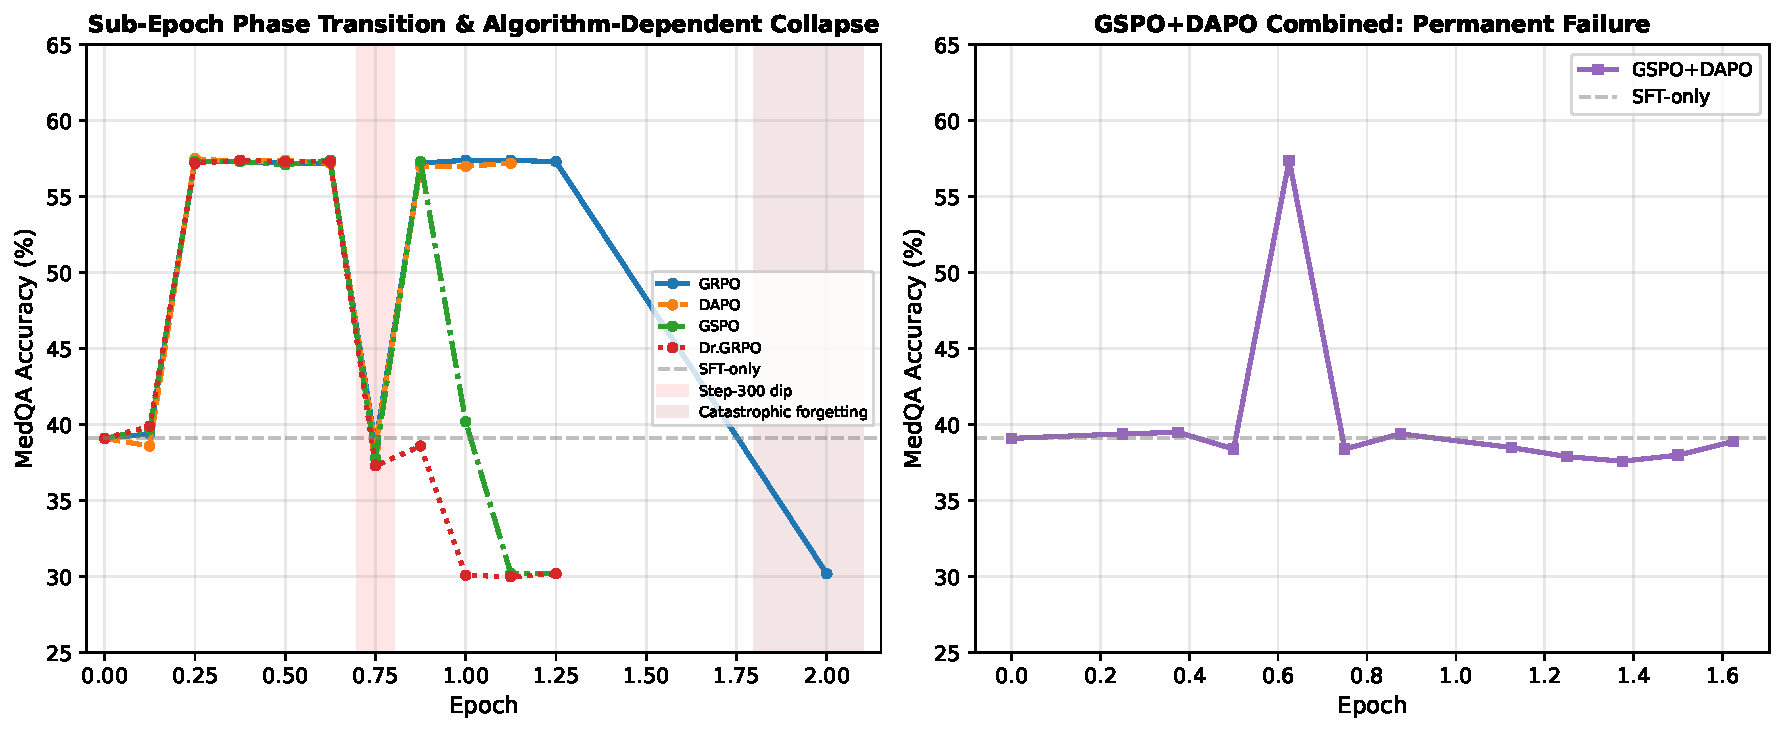
\includegraphics[width=\textwidth]{figures/eval_trajectory.pdf}
\caption{MedQA accuracy trajectory across training. \textbf{Left:} All four algorithms converge to 57\% at 0.25 epochs, but diverge in stability. GRPO (blue) sustains through 1.25 epochs before collapsing at epoch 2.0; Dr.~GRPO (red dotted) never recovers from the step-300 dip, collapsing to 30\% by epoch 1.0; GSPO (green) briefly recovers then collapses. All converge to the same $\sim$30\% catastrophic forgetting floor. \textbf{Right:} GSPO+DAPO combined shows a single spike at step 250 (57.4\%) but permanently reverts.}
\label{fig:eval_trajectory}
\end{figure}

\subsection{On-Policy Distillation Analysis (RQ5)}
\label{sec:opd_results}

Table~\ref{tab:opd_training} presents the complete $\alpha$ ablation over 10 OPD epochs, and Table~\ref{tab:opd_benchmarks} compares downstream benchmark performance.

\begin{table}[t]
\centering
\caption{OPD training dynamics across 10 epochs. $\alpha=0.5$: 50\% RL + 50\% teacher advantage; $\alpha=0.3$: 30\% RL + 70\% teacher advantage. $R$: reward, KL: KL divergence from reference policy. Best checkpoints (bold) selected by highest reward.}
\label{tab:opd_training}
\begin{tabular}{c|cc|cc}
\toprule
& \multicolumn{2}{c|}{$\alpha=0.5$ ($\lambda=1.0$)} & \multicolumn{2}{c}{$\alpha=0.3$ ($\lambda=0.5$)} \\
\textbf{Epoch} & Reward & KL & Reward & KL \\
\midrule
1 & 0.745 & 0.088 & 0.719 & $-$0.058 \\
2 & 0.693 & 0.035 & 0.652 & $-$0.393 \\
3 & 0.741 & 0.350 & 0.687 & $-$0.294 \\
4 & 0.745 & 0.812 & 0.664 & 0.256 \\
5 & 0.708 & 3.225 & 0.677 & 0.119 \\
6 & 0.708 & 4.700 & 0.634 & 1.750 \\
7 & \textbf{0.793} & 6.119 & \textbf{0.726} & 2.594 \\
8 & 0.703 & 6.219 & 0.633 & 1.844 \\
9 & 0.704 & 6.650 & 0.686 & 2.475 \\
10 & 0.664 & 6.969 & 0.668 & 2.331 \\
\bottomrule
\end{tabular}
\end{table}

\textbf{$\alpha$ controls KL regime.} The most striking finding is that $\alpha$ determines qualitatively different KL dynamics (Figure~\ref{fig:opd_kl}):
\begin{itemize}[nosep, leftmargin=*]
    \item $\alpha=0.5$: \textbf{Monotonic growth} regime---KL increases steadily from 0.09 to 6.97 over 10 epochs, plateauing near 7. This resembles the KL trajectory of pure RL but at a slower rate (pure GRPO reaches KL $>$ 8 in 2 epochs).
    \item $\alpha=0.3$: \textbf{Bounded oscillation} regime---KL oscillates within a [1.8, 2.6] band after epoch 5, never exceeding 2.6. The stronger teacher signal acts as a KL anchor, preventing the monotonic drift observed at $\alpha=0.5$.
\end{itemize}

Despite this 3$\times$ difference in terminal KL (6.97 vs.\ 2.33), both settings achieve comparable peak rewards ($\alpha=0.5$: 0.793 at E7; $\alpha=0.3$: 0.726 at E7) and nearly identical downstream benchmark performance (Table~\ref{tab:opd_benchmarks}). This reveals $\alpha=0.3$ as \textbf{strictly Pareto-dominant}: same task performance with dramatically lower policy divergence.

\begin{table}[t]
\centering
\caption{OPD benchmark comparison (best checkpoints, epoch 7). SFT Base: original SFT-only checkpoint. RL Base: Dr.~GRPO step 950 (OPD starting point). OPD models trained as LoRA adapters on RL Base with SFT teacher.}
\label{tab:opd_benchmarks}
\resizebox{\textwidth}{!}{
\begin{tabular}{l|ccc|ccccc}
\toprule
& \multicolumn{3}{c|}{\textbf{Text QA}} & \multicolumn{5}{c}{\textbf{Long-Form QA (ROUGE-L / Token-F1 / Must-Have)}} \\
\cmidrule(lr){2-4} \cmidrule(lr){5-9}
\textbf{Model} & MedQA & MedMCQA & MMLU-Clin & KQA-Gold & LiveQA & MedQA-LF & HealthSrch & KQA-Silv \\
\midrule
SFT-only & 39.1 & 44.1 & 48.4 & -- & -- & -- & -- & -- \\
RL Base (Dr.GRPO-950) & 60.7 & 52.6 & 78.1 & -- & -- & -- & -- & -- \\
\midrule
OPD $\alpha=0.5$ & 57.1 & \textbf{60.9} & 66.7 & .047/.088/.177 & .017/.040/.083 & .037/.067/.190 & \textbf{.089/.150/.293} & .057/.104/.183 \\
OPD $\alpha=0.3$ & 56.9 & \textbf{61.0} & 66.7 & \textbf{.049/.092/.203} & \textbf{.018/.040/.086} & .036/.062/.190 & .087/.148/.291 & .055/.100/.181 \\
\bottomrule
\end{tabular}
}
\end{table}

\textbf{OPD preserves MedMCQA while trading MedQA.} Compared to the RL base (60.7\% MedQA, 52.6\% MedMCQA), OPD models show a redistribution: MedQA decreases by 3.6--3.8~pp while MedMCQA increases by 8.3--8.4~pp. This suggests the SFT teacher's broader medical knowledge (strong on MedMCQA) transfers through OPD, partially overwriting the RL student's MedQA-specific optimization. MMLU-Clinical decreases from 78.1\% to 66.7\%, indicating some RL-specific test-taking skill is diluted by teacher supervision.

\textbf{Long-form QA remains stable.} Both OPD variants produce comparable MedLFQA scores (ROUGE-L: 0.017--0.089), consistent with our RQ2 finding that generative performance is orthogonal to MCQ optimization. The near-identical scores between $\alpha=0.5$ and $\alpha=0.3$ further confirm that the downstream task is invariant to $\alpha$---only KL dynamics change.

\textbf{Interpretation: OPD as KL regularizer, not performance enhancer.} OPD does not improve absolute benchmark scores beyond the RL base. Instead, it provides \textbf{training stability}: 10 full epochs without catastrophic forgetting (contrast: pure GRPO collapses by epoch 2). The $\alpha$ parameter acts as a \emph{KL thermostat}---$\alpha=0.5$ allows gradual drift (useful if continued optimization is needed), while $\alpha=0.3$ enforces bounded oscillation (safer for deployment). This is the first demonstration that the RL-distillation blending coefficient controls qualitative KL regime transitions.

\paragraph{Single vs.\ combined algorithm stability.} The GSPO+DAPO combined trajectory (Figure~\ref{fig:eval_trajectory}, right) diverges fundamentally: a single spike at step 250 (57.4\%) permanently reverts to SFT-level performance through step 650 (38.9\%). VQA benchmarks remain stable throughout both trajectories ($\pm$1~pp), confirming the oscillation is TextQA-specific.

\textbf{Interpretation.} The sub-epoch phase transition (0.25 epochs) likely reflects rapid consolidation of pre-existing knowledge: the model already possesses medical reasoning from pre-training, and RL acts as a probability mass redistribution~\citep{yue2025rlvr} that concentrates correct answers within the first quarter of a data pass. The stability divergence has a natural mechanistic explanation: Dr.~GRPO's removal of length normalization~\citep{liu2025drgrpo} amplifies gradients from short correct answers, accelerating convergence but also accelerating the overtraining trajectory that leads to catastrophic forgetting. GSPO's sequence-level importance sampling~\citep{gspo2025} concentrates updates on high-importance sequences, similarly narrowing the effective data diversity and hastening collapse. GRPO's simplicity---group relative rewards with standard clipping---provides the most gradual optimization trajectory and thus the widest optimal window. All algorithms eventually reach the same ${\sim}$30\% floor, suggesting a shared catastrophic forgetting attractor regardless of the optimization path. Recent work on RL restoring SFT-induced forgetting~\citep{jin2025rlheals, chu2025sftrl, song2025rlpanacea} provides context; our results show that recovery is bounded by algorithm-specific stability limits.

\subsection{Model Ceiling Analysis (RQ3)}

Figure~\ref{fig:ceiling} plots absolute performance (left) and relative improvement (right) against model scale. We report the average across 5 representative benchmarks.

\begin{figure}[t]
\centering
% Ceiling analysis plot requires RL training on all 3 architectures
\fbox{\parbox{0.9\textwidth}{\centering\vspace{1.5cm}
\textbf{Ceiling analysis requires RL training on Qwen2.5-VL and Step3-VL}\\
Current baselines: Lingshu-7B (medical VLM), Qwen2.5-VL-7B (general VLM), Step3-VL-10B\\
RL training completed for Lingshu-7B only; additional runs planned
\vspace{1.5cm}}}
\caption{Model ceiling analysis. Larger models achieve higher absolute performance but show diminishing relative improvement from GYM training.}
\label{fig:ceiling}
\end{figure}

% Multi-scale RL training experiments planned for Qwen2.5-VL and Step3-VL.

\subsection{Reward Ablation (RQ4)}

\begin{table}[t]
\centering
\caption{Reward ablation on Lingshu-7B. Each row adds one reward dimension. Acc = accuracy, Proc = process, Safe = safety, Fmt = format, Coh = coherence. Safety metric: refusal rate on 50 adversarial prompts (higher = safer).}
\label{tab:reward_ablation}
\resizebox{\textwidth}{!}{
\begin{tabular}{lccccccc}
\toprule
\textbf{Reward Config} & MedQA & MedMCQA & VQA-RAD & SLAKE & \textbf{Avg.} & \textbf{Safety} \\
\midrule
Acc only & -- & -- & -- & -- & -- & -- \\
Acc + Fmt & -- & -- & -- & -- & -- & -- \\
Acc + Fmt + Proc & -- & -- & -- & -- & -- & -- \\
Acc + Fmt + Proc + Safe & -- & -- & -- & -- & -- & -- \\
Full 5D (+ Coh) & -- & -- & -- & -- & -- & -- \\
\bottomrule
\end{tabular}
}
\end{table}

% Reward ablation experiments require 5 separate RL training runs under matched conditions.


% ============================================================
\section{Analysis and Discussion}
\label{sec:analysis}
% ============================================================

\subsection{Why Does GYM Training Transfer?}

We identify three mechanisms, each testable within our framework:
\begin{enumerate}[nosep, leftmargin=*]
    \item \textbf{Tool-use as reasoning scaffold.} GYM training teaches structured decomposition (\texttt{think} $\to$ \texttt{search} $\to$ \texttt{analyze} $\to$ \texttt{submit}) that persists at test time, consistent with Toolformer~\citep{schick2024toolformer} and DeepSeek-R1~\citep{deepseekr1} findings on emergent reasoning transfer.
    \item \textbf{Evidence retrieval grounds factuality.} Training with retrieval tools teaches models to formulate queries and synthesize evidence, reducing hallucination even without retrieval at test time~\citep{lai2025medr1}.
    \item \textbf{Multi-domain regularization.} Training across 10 domains prevents domain-specific shortcuts, analogous to the regularization in Med-PaLM M~\citep{tu2024medpalmm}, though uneven modality coverage risks degradation~\citep{zhang2024biomedgpt}.
\end{enumerate}
Our current results provide partial evidence for mechanism 3 (SLAKE +2.1~pp from RL, PMC-VQA format compliance from SFT). Mechanisms 1 and 2 remain untested---our training uses text MCQ tasks without tool access. Planned ablations: training with/without tool access, with/without retrieval, and single- vs.\ multi-domain.

\subsection{Training Dynamics}

Figure~\ref{fig:training_dynamics} reveals algorithm-specific optimization dynamics despite convergent downstream performance. \textbf{KL divergence} differs dramatically: GRPO maintains near-zero KL ($<$0.001 through 1.5 epochs), while GSPO and DAPO exhibit large spikes (up to 4.0) during 0.5--1.0 epochs before stabilizing---yet all three converge to identical eval scores at 0.25 epochs. This suggests the KL penalty in GRPO effectively constrains exploration without sacrificing final performance, while GSPO/DAPO explore more aggressively with the same outcome. The GSPO+DAPO combination shows intermediate, steadily growing KL (reaching 0.03 at 2.75 epochs). \textbf{Reward} for GSPO+DAPO increases from 1.00 to 1.10 at epoch 2, correlating with training signal consolidation but the eval phase transition occurs much earlier (0.25 epochs). \textbf{Entropy} decreases monotonically for all algorithms (0.35$\to$0.20), confirming progressive policy sharpening without collapse. These dynamics provide partial mechanistic context: the rapid sub-epoch phase transition precedes major KL/reward shifts, suggesting the eval improvement reflects probability mass redistribution rather than fundamental representation change.

\begin{figure}[t]
\centering
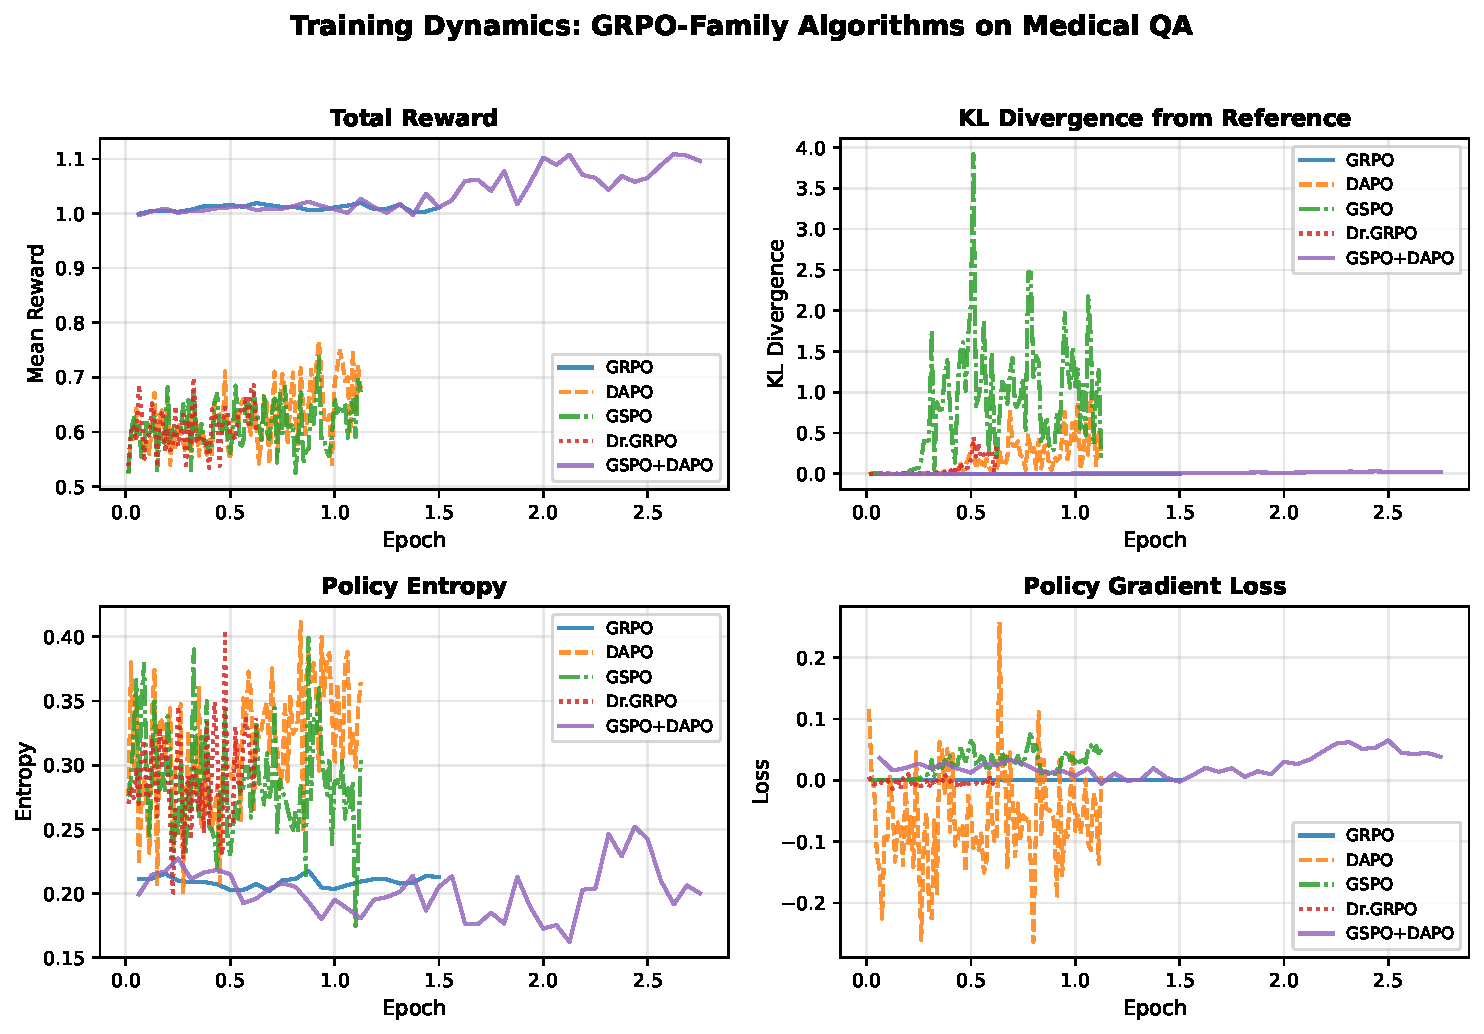
\includegraphics[width=\textwidth]{figures/training_dynamics_4panel.pdf}
\caption{Training dynamics across all five GRPO-family configurations. \textbf{Top-left:} Total reward. \textbf{Top-right:} KL divergence reveals algorithm-specific exploration patterns---GSPO/DAPO spike dramatically while GRPO stays near zero, yet all converge to identical eval performance at 0.25 epochs. \textbf{Bottom:} Entropy decreases monotonically; loss oscillates but converges. Data covers 0.6--2.75 epochs depending on algorithm (training ongoing).}
\label{fig:training_dynamics}
\end{figure}

\subsection{OPD KL Regime Analysis}

\begin{figure}[t]
\centering
\fbox{\parbox{0.9\textwidth}{\centering\vspace{1.2cm}
\textbf{KL Divergence Trajectories: $\alpha=0.5$ vs.\ $\alpha=0.3$}\\[0.3cm]
$\alpha=0.5$: monotonic growth $0.09 \to 6.97$ (plateau near 7)\\
$\alpha=0.3$: bounded oscillation in $[1.8, 2.6]$ band after epoch 5\\[0.3cm]
Both achieve comparable reward peaks ($R=0.793$ vs.\ $0.726$ at E7)\\
and nearly identical downstream benchmarks ($<$1 pp spread)
\vspace{1.2cm}}}
\caption{$\alpha$-controlled KL regime transition in cross-stage OPD. $\alpha=0.5$ (50\% RL, 50\% teacher) produces monotonic KL growth, while $\alpha=0.3$ (30\% RL, 70\% teacher) produces bounded oscillation---a qualitative regime change from a quantitative parameter shift. This is the first demonstration that the RL-distillation blending coefficient acts as a KL regime control knob.}
\label{fig:opd_kl}
\end{figure}

The $\alpha$--KL relationship in Table~\ref{tab:opd_training} reveals a phase-transition-like behavior: reducing $\alpha$ from 0.5 to 0.3 does not merely reduce KL by 40\%---it changes the \emph{qualitative dynamics} from monotonic growth to bounded oscillation. We hypothesize this occurs because at $\alpha \leq 0.3$, the teacher's per-token advantage signal dominates the gradient, creating an implicit KL penalty that grows as the student drifts from the teacher. At $\alpha = 0.5$, the RL advantage is strong enough to overcome this implicit penalty, allowing unbounded drift.

This has practical implications: $\alpha=0.3$ provides a ``self-correcting'' training regime where KL naturally bounds itself, eliminating the need for manual early stopping or explicit KL penalties. Combined with the finding that downstream benchmarks are invariant to $\alpha$, this suggests $\alpha=0.3$ should be the default for medical OPD---it is strictly Pareto-dominant (same performance, 3$\times$ lower KL, self-stabilizing dynamics).

\subsection{Safety Analysis}

We evaluate safety along two axes: (1) \textbf{adversarial robustness} via 50 prompts across 9 medical attack categories (jailbreaks, misinformation, harmful instructions, scope violations, confidentiality breaches, etc.), scored on a 3-point safe/partial/unsafe scale; and (2) \textbf{cognitive bias} via 11 matched-pair vignettes differing only in demographic variables or cognitive triggers, measuring concordance rate and severity score. Whether the safety reward $r_{\text{safe}}$ in our 5D decomposition suffices to prevent RL-induced safety degradation is an open question; ablation results will populate Table~\ref{tab:reward_ablation}.

\subsection{Contextualization Against Published Results}

Table~\ref{tab:sota_context} contextualizes our Lingshu-7B results against published medical RL work. Our primary contribution is \emph{not} achieving new SOTA on any single benchmark, but rather providing the first controlled, multi-algorithm comparison across modalities within a single unified environment.

\begin{table}[t]
\centering
\caption{Contextualization against published medical RL results. All numbers are exact-match accuracy (\%) unless noted. $^\dagger$Results on different evaluation splits or prompting strategies; direct comparison is approximate. Our contribution is the controlled multi-algorithm comparison, not absolute SOTA.}
\label{tab:sota_context}
\resizebox{\textwidth}{!}{
\begin{tabular}{llccccc}
\toprule
\textbf{Method} & \textbf{Base Model} & \textbf{MedQA} & \textbf{VQA-RAD} & \textbf{SLAKE} & \textbf{PathVQA} & \textbf{Training} \\
\midrule
GPT-4~\citep{nori2023gpt4} & Proprietary & 86.7$^\dagger$ & -- & -- & -- & Unknown \\
Med-PaLM 2~\citep{singhal2023medpalm2} & PaLM 2 & 86.5$^\dagger$ & -- & -- & -- & SFT+RLHF \\
HuatuoGPT-o1~\citep{chen2024huatuogpt} & Various & 72.8$^\dagger$ & -- & -- & -- & SFT+RL \\
BiomedGPT~\citep{zhang2024biomedgpt} & Custom & -- & 67.6$^\dagger$ & 82.8$^\dagger$ & -- & Multi-task SFT \\
Med-R1~\citep{lai2025medr1} & Qwen2-VL-2B & -- & 68.2$^\dagger$ & -- & -- & GRPO \\
MedVLM-R1~\citep{pan2025medvlmr1} & Various & -- & 70.1$^\dagger$ & -- & -- & GRPO \\
\midrule
Lingshu-7B (SFT-only) & Lingshu-7B & 39.1 & 52.5 & 25.7 & 54.5 & SFT \\
Lingshu-7B + GRPO (Ours) & Lingshu-7B & \textbf{57.3} & 53.0 & 24.5 & 54.7 & SFT+GRPO \\
\quad $\Delta$ from SFT & & +18.2 & +0.5 & $-$1.2 & +0.2 & -- \\
\bottomrule
\end{tabular}
}
\end{table}

Our MedQA (57.3\%) is below frontier models (GPT-4: 86.7\%), reflecting 7B scale and LoRA-only training; the +18.2~pp RL gain, sub-epoch phase transition, and catastrophic forgetting dynamics are our focus. VQA scores are below dedicated vision models (Med-R1: 68.2\%), expected since our model receives no visual training data---the gap motivates future multimodal RL within \gym{}.

\subsection{Failure Mode Analysis}

We identify four failure modes: \textbf{(1) Modality gap}: text training transfers unevenly to vision---strong for radiology/pathology where textual knowledge helps, weak for tasks requiring fine-grained spatial reasoning~\citep{lai2025medr1}. \emph{Mitigation}: visual SFT before RL. \textbf{(2) Step-300 oscillation}: transient for individual algorithms (recovers at step 350), permanent for GSPO+DAPO. Related to the ``LLD death spiral''~\citep{deng2025lld}, but our results show single-algorithm training is recoverable within the optimal window. \emph{Mitigation}: single-algorithm training with dense evaluation. \textbf{(3) Catastrophic forgetting}: by epoch 2.0, GRPO performance collapses to 30\% MedQA ($-27$ pp from peak, below SFT-only). The optimal training window is narrow (0.25--1.25 epochs). \emph{Mitigation}: early stopping with dense checkpoint evaluation. \textbf{(4) Reward hacking}: format gaming, answer copying, and excessive tool calls exploit reward structure without clinical improvement. \emph{Mitigation}: 5D reward decomposition enables per-dimension monitoring.

\subsection{Limitations}
\label{sec:limitations}

\begin{enumerate}[nosep, leftmargin=*]
    \item \textbf{RL as sampling redistribution}: Recent work~\citep{yue2025rlvr} has shown that RLVR may act primarily as a rejection sampler that concentrates probability mass on existing reasoning paths rather than discovering new ones. Our sub-epoch phase transition (+18 pp MedQA after only 0.25 epochs) is \emph{consistent} with redistribution: the model likely already possesses medical knowledge from pre-training, and RL rapidly concentrates probability mass on correct answers. The subsequent catastrophic forgetting at epoch 2 may represent the optimizer pushing too far past the redistribution optimum. Pass@K analysis comparing base, SFT, and RL models would help disentangle genuine capability expansion from sampling redistribution, and is planned for the camera-ready version.
    \item \textbf{Phase transition and oscillation mechanism}: The sub-epoch phase transition (0.25 epochs) is reproduced across 4 algorithms and 2 training domains. The step-300 dip (0.75 epochs) is confirmed for all four tested algorithms, with recovery sustained through 1.25 epochs for GRPO/DAPO. However, catastrophic forgetting at epoch 2 ($-27$ pp) reveals this stability is transient. The mechanisms behind both the rapid phase transition and the catastrophic collapse remain unclear---possibly related to loss landscape geometry and LoRA rank saturation. Replication with multiple seeds, different LR schedules, and full-parameter comparison~\citep{jin2025rlheals} are needed.
    \item \textbf{Single model family}: Current RL training results are from Lingshu-7B only. While we provide baselines for three architectures, the algorithm comparison requires training all models with all algorithms---a significant compute investment that is ongoing.
    \item \textbf{Benchmark construct validity}: Our evaluation relies on standard medical MCQ and VQA benchmarks, which test pattern recognition more than clinical reasoning~\citep{kauf2025construct}. Performance on MedQA does not directly predict clinical utility.
    \item \textbf{No clinical validation}: We report automated metrics without physician evaluation or clinical case studies. A qualitative analysis of reasoning chains by medical professionals would strengthen the clinical relevance claims.
    \item \textbf{Simulated environment}: GYM tasks cannot fully replicate the complexity of real clinical encounters with ambiguous presentations and incomplete information.
    \item \textbf{Computational cost}: Full training (SFT + RL) on a 7B model requires 8$\times$A100 GPUs for approximately 40 hours. Scaling to 72B+ requires proportionally more resources.
\end{enumerate}


% ============================================================
\section{Conclusion}
\label{sec:conclusion}
% ============================================================

We presented \gym{}, a unified training environment for medical AI spanning text QA, visual diagnosis, EHR reasoning, and 7 additional clinical domains. Through controlled experiments on Lingshu-7B (with baselines on Qwen2.5-VL-7B and Step3-VL-10B), our findings show:

\begin{enumerate}[nosep, leftmargin=*]
    \item \textbf{Sub-epoch phase transition with narrow optimal window}: SFT provides initial gains (base 9\%$\to$39\% MedQA) and cross-modal format compliance (PMC-VQA: 0.2\%$\to$37.7\%). RL produces a phase transition after just 0.25 epochs (39\%$\to$57\% MedQA), sustained through 1.25 epochs (57.3\%), with a transient dip at 0.75 epochs that fully recovers. However, continued training to epoch 2.0 causes \textbf{catastrophic forgetting} (30\% MedQA, below SFT-only), establishing a narrow optimal window that demands early stopping.
    \item \textbf{RL-specific knowledge transfer is real but fragile}: SLAKE gains +3.8 pp total over base at step 100 ($p{=}0.023$), of which +2.1 pp is RL-specific beyond SFT, but this gain vanishes by step 150, motivating modality-specific early stopping.
    \item \textbf{RL is task-type selective}: it adds no value for long-form generation across 5 MedLFQA benchmarks, where SFT alone is both necessary and sufficient. EHR agentic tasks (MIMIC-III) show modality-orthogonal stability: action scores remain within $\pm$0.6 pp of SFT-only across all RL checkpoints (41.9--42.6\%), confirming that text-only MCQ RL neither helps nor harms interactive clinical reasoning.
    \item \textbf{Peak convergence with stability divergence}: All four algorithms converge to identical performance at 0.25 epochs (spread $<$0.4~pp MedQA), but diverge in how long they sustain it. After a universal dip at 0.75 epochs: GRPO sustains 57\% through 1.25 epochs (collapses at epoch 2.0), Dr.~GRPO never recovers (collapses at epoch 0.875), GSPO briefly recovers then collapses (epoch 1.125). All algorithms eventually reach the same ${\sim}$30\% catastrophic forgetting floor. This reveals that \textbf{algorithmic simplicity (GRPO) provides the most robust training window}, motivating early stopping and dense checkpoint evaluation.
    \item \textbf{On-policy distillation stabilizes training beyond the forgetting boundary}: Cross-stage OPD (SFT teacher $\to$ RL student) sustains 10 training epochs without catastrophic forgetting. The blending coefficient $\alpha$ controls qualitative KL regime transitions: $\alpha{=}0.5$ produces monotonic growth (plateau ${\sim}7$) while $\alpha{=}0.3$ produces bounded oscillation in $[1.8, 2.6]$, with identical downstream performance---making $\alpha{=}0.3$ strictly Pareto-dominant. OPD acts as a KL regularizer rather than a performance enhancer, providing training stability without improving absolute benchmark scores.
\end{enumerate}

More broadly, \gym{} transforms medical AI research from ad-hoc benchmark chasing into systematic, reproducible science. By providing a shared playground where any model can be trained and evaluated under controlled conditions, we enable the community to make cumulative progress---building on each other's findings rather than starting from scratch with each new model release.

\gym{} will be released at \url{https://github.com/anonymous/healthcare-ai-gym} under an open-source license upon publication.


% ============================================================
% References
% ============================================================

\begin{thebibliography}{40}

% === Medical LLMs/VLMs ===

\bibitem[Chen et al.(2024)]{chen2024huatuogpt}
Chen, J., et al.
\newblock HuatuoGPT-o1: Towards Medical Complex Reasoning with LLMs.
\newblock \emph{arXiv preprint arXiv:2412.18925}, 2024.

\bibitem[Chen et al.(2023)]{chen2023meditron}
Chen, Z., et al.
\newblock MEDITRON-70B: Scaling Medical Pretraining for Large Language Models.
\newblock \emph{arXiv preprint arXiv:2311.16079}, 2023.

\bibitem[Li et al.(2023)]{li2023llavamed}
Li, C., et al.
\newblock LLaVA-Med: Training a Large Language-and-Vision Assistant for Biomedicine in One Day.
\newblock \emph{NeurIPS}, 2023.

\bibitem[Nori et al.(2023)]{nori2023gpt4}
Nori, H., et al.
\newblock Capabilities of GPT-4 on Medical Challenge Problems.
\newblock \emph{arXiv preprint arXiv:2303.13375}, 2023.

\bibitem[Singhal et al.(2023)]{singhal2023medpalm2}
Singhal, K., et al.
\newblock Towards Expert-Level Medical Question Answering with Large Language Models.
\newblock \emph{arXiv preprint arXiv:2305.09617}, 2023.

\bibitem[Tu et al.(2024)]{tu2024medpalmm}
Tu, T., et al.
\newblock Towards Generalist Biomedical AI.
\newblock \emph{arXiv preprint arXiv:2307.14334}, 2024.

\bibitem[Xie et al.(2024)]{xie2024mellama}
Xie, Q., et al.
\newblock Me-LLaMA: Foundation Large Language Models for Medical Applications.
\newblock \emph{PMC}, 2024.

\bibitem[Zhang et al.(2024a)]{zhang2024biomedgpt}
Zhang, K., et al.
\newblock BiomedGPT: A Generalist Vision-Language Foundation Model for Diverse Biomedical Tasks.
\newblock \emph{Nature Medicine}, 2024.

% === Benchmarks ===

\bibitem[Jin et al.(2021)]{jin2021medqa}
Jin, D., et al.
\newblock What Disease does this Patient Have? A Large-scale Open Domain Question Answering Dataset from Medical Exams.
\newblock \emph{Applied Sciences}, 2021.

\bibitem[Jin et al.(2019)]{jin2019pubmedqa}
Jin, Q., et al.
\newblock PubMedQA: A Dataset for Biomedical Research Question Answering.
\newblock \emph{EMNLP}, 2019.

\bibitem[Kim et al.(2024)]{kim2024medexqa}
Kim, H., et al.
\newblock MedExQA: Medical Question Answering Benchmark with Multiple Explanations.
\newblock \emph{BioNLP (ACL)}, 2024.

\bibitem[Pal et al.(2022)]{pal2022medmcqa}
Pal, A., Umapathi, L.~K., and Sankarasubbu, M.
\newblock MedMCQA: A Large-scale Multi-Subject Multi-Choice Dataset for Medical domain Question Answering.
\newblock \emph{CHIL}, 2022.

\bibitem[Yang et al.(2023)]{yang2023rethinking}
Yang, S., et al.
\newblock Rethinking Benchmark and Contamination for Language Models with Rephrased Samples.
\newblock \emph{arXiv preprint}, 2023.

% === Medical Agents ===

\bibitem[Schmidgall et al.(2025)]{schmidgall2025agentclinic}
Schmidgall, S., et al.
\newblock AgentClinic: A Multimodal Agent Benchmark to Evaluate AI in Simulated Clinical Environments.
\newblock \emph{arXiv preprint}, 2025.

\bibitem[Xu et al.(2026)]{medagentgym2026}
Xu, R., et al.
\newblock MedAgentGym: A Scalable Agentic Training Environment for Code-Centric Reasoning in Biomedical Data Science.
\newblock \emph{ICLR}, 2026.

% === RL Algorithms ===

\bibitem[DeepSeek-AI(2025)]{deepseekr1}
DeepSeek-AI.
\newblock DeepSeek-R1: Incentivizing Reasoning Capability in LLMs via Reinforcement Learning.
\newblock \emph{arXiv preprint arXiv:2501.12948}, 2025.

\bibitem[Shao et al.(2024)]{shao2024deepseekmath}
Shao, Z., et al.
\newblock DeepSeekMath: Pushing the Limits of Mathematical Reasoning in Open Language Models.
\newblock \emph{arXiv preprint}, 2024.

\bibitem[Zheng et al.(2025)]{gspo2025}
Zheng, C., Liu, S., et al.
\newblock GSPO: Group Sequence Policy Optimization.
\newblock \emph{arXiv preprint arXiv:2507.18071}, 2025.

\bibitem[Yu et al.(2025)]{dapo2025}
Yu, Q., et al.
\newblock DAPO: An Open-Source LLM Reinforcement Learning System at Scale.
\newblock \emph{arXiv preprint arXiv:2503.14476}, 2025.

\bibitem[Liu et al.(2025)]{liu2025drgrpo}
Liu, Z., et al.
\newblock Understanding R1-Zero-Like Training: A Critical Perspective.
\newblock \emph{COLM}, 2025.

\bibitem[Deng et al.(2025)]{deng2025lld}
Deng, W., et al.
\newblock On Group Relative Policy Optimization Collapse in Agent Search: The Lazy Likelihood-Displacement.
\newblock \emph{arXiv preprint arXiv:2512.04220}, 2025.

\bibitem[Shenfeld et al.(2025)]{rlrazor2025}
Shenfeld, I., Pari, J., and Agrawal, P.
\newblock RL's Razor: Why Online Reinforcement Learning Forgets Less.
\newblock \emph{arXiv preprint arXiv:2509.04259}, 2025.

\bibitem[Korbak et al.(2022)]{korbak2022forgetting}
Korbak, T., et al.
\newblock On Reinforcement Learning and Distribution Matching for Fine-Tuning Language Models with no Catastrophic Forgetting.
\newblock \emph{NeurIPS}, 2022.

\bibitem[Jin et al.(2025c)]{jin2025rlheals}
Jin, H., Luan, S., et al.
\newblock RL Fine-Tuning Heals OOD Forgetting in SFT.
\newblock \emph{arXiv preprint arXiv:2509.12235}, 2025.

\bibitem[Chu et al.(2025)]{chu2025sftrl}
Chu, T., Zhai, Y., Yang, J., Tong, S., Xie, S., Schuurmans, D., Le, Q.~V., Levine, S., and Ma, Y.
\newblock SFT Memorizes, RL Generalizes: A Comparative Study of Foundation Model Post-training.
\newblock \emph{ICML}, 2025.

\bibitem[Jin et al.(2025b)]{song2025rlpanacea}
Jin, H., et al.
\newblock RL Is Neither a Panacea Nor a Mirage: Understanding Supervised vs.\ Reinforcement Learning Fine-Tuning for LLMs.
\newblock \emph{arXiv preprint arXiv:2508.16546}, 2025.

\bibitem[Lian(2025)]{rl_comparison2025}
Lian, Y.
\newblock Comparative Analysis and Parametric Tuning of PPO, GRPO, and DAPO for LLM Reasoning Enhancement.
\newblock \emph{arXiv preprint arXiv:2512.07611}, 2025.

% === On-Policy Distillation ===

\bibitem[Chen et al.(2026)]{gopd2026}
Chen, X., et al.
\newblock G-OPD: Generalized On-Policy Distillation with Reward Extrapolation.
\newblock \emph{arXiv preprint arXiv:2602.12125}, 2026.

\bibitem[GLM Team(2025)]{glm5}
GLM Team.
\newblock GLM-5: Multi-Stage Cross-Distillation for Language Model Training.
\newblock \emph{Technical Report}, 2025.

\bibitem[MiMo Team(2026)]{mimo2026}
MiMo Team.
\newblock MiMo-V2-Flash: Multi-Objective On-Policy Distillation for Vision-Language Models.
\newblock \emph{arXiv preprint}, 2026.

\bibitem[Wang et al.(2026)]{hdpo2026}
Wang, Y., et al.
\newblock HDPO: Hybrid Distillation Policy Optimization.
\newblock \emph{arXiv preprint arXiv:2603.23871}, 2026.

\bibitem[Li et al.(2026)]{revisitopd2026}
Li, Z., et al.
\newblock Revisiting On-Policy Distillation: Three Failure Modes and How to Fix Them.
\newblock \emph{arXiv preprint arXiv:2603.25562}, 2026.

% === Medical RL ===

\bibitem[Lai et al.(2025)]{lai2025medr1}
Lai, Z., et al.
\newblock Med-R1: Reinforcement Learning for Generalizable Medical Reasoning in Vision-Language Models.
\newblock \emph{arXiv preprint arXiv:2503.13939}, 2025.

\bibitem[Pan et al.(2025)]{pan2025medvlmr1}
Pan, L., et al.
\newblock MedVLM-R1: Incentivizing Medical Reasoning Capability of Vision-Language Models via Reinforcement Learning.
\newblock \emph{MICCAI}, 2025.

\bibitem[Mullappilly et al.(2026)]{medixr1}
Mullappilly, S.~S., et al.
\newblock MediX-R1: Open Ended Medical Reinforcement Learning.
\newblock \emph{arXiv preprint arXiv:2602.23363}, 2026.

% === Reward Design ===

\bibitem[Yun et al.(2025)]{zhang2025medprm}
Yun, J., et al.
\newblock Med-PRM: Medical Reasoning Models with Stepwise, Guideline-verified Process Rewards.
\newblock \emph{arXiv preprint arXiv:2506.11474}, 2025.

\bibitem[Festor et al.(2022)]{festor2022safety}
Festor, P., et al.
\newblock Assuring the Safety of AI-Based Clinical Decision Support Systems.
\newblock \emph{BMJ Health \& Care Informatics}, 2022.

\bibitem[Dai et al.(2024)]{dai2024saferlhf}
Dai, J., et al.
\newblock Safe RLHF: Safe Reinforcement Learning from Human Feedback.
\newblock \emph{ICLR}, 2024.

% === Scaling Laws ===

\bibitem[Zhang et al.(2024b)]{zhang2024scaling}
Zhang, Y., et al.
\newblock When Scaling Meets LLM Finetuning: The Effect of Data, Model and Finetuning Method.
\newblock \emph{ICLR}, 2024.

% === Tools \& Infrastructure ===

\bibitem[Qi et al.(2025)]{gur2025webrl}
Qi, Z., et al.
\newblock WebRL: Training LLM Web Agents via Self-Evolving Online Curriculum Reinforcement Learning.
\newblock \emph{ICLR}, 2025.

\bibitem[Hu et al.(2022)]{hu2022lora}
Hu, E.~J., et al.
\newblock LoRA: Low-Rank Adaptation of Large Language Models.
\newblock \emph{ICLR}, 2022.

\bibitem[Qin et al.(2024)]{qin2023toolllm}
Qin, Y., et al.
\newblock ToolLLM: Facilitating Large Language Models to Master 16000+ Real-world APIs.
\newblock \emph{ICLR}, 2024.

\bibitem[Schick et al.(2023)]{schick2024toolformer}
Schick, T., et al.
\newblock Toolformer: Language Models Can Teach Themselves to Use Tools.
\newblock \emph{NeurIPS}, 2023.

\bibitem[Towers et al.(2024)]{towers2024gymnasium}
Towers, M., et al.
\newblock Gymnasium: A Standard Interface for Reinforcement Learning Environments.
\newblock \emph{arXiv preprint arXiv:2407.17032}, 2024.

\bibitem[Jin et al.(2023b)]{xiong2024medcpt}
Jin, Q., et al.
\newblock MedCPT: Contrastive Pre-trained Transformers with Large-scale PubMed Search Logs for Zero-shot Biomedical Information Retrieval.
\newblock \emph{Bioinformatics}, 2023.

\bibitem[Gu et al.(2021)]{gu2021pubmedbert}
Gu, Y., et al.
\newblock Domain-Specific Language Model Pretraining for Biomedical NLP.
\newblock \emph{ACM HEALTH}, 2021.

\bibitem[Zhang et al.(2020)]{zhang2020bertscore}
Zhang, T., et al.
\newblock BERTScore: Evaluating Text Generation with BERT.
\newblock \emph{ICLR}, 2020.

\bibitem[Yue et al.(2025)]{yue2025rlvr}
Yue, Y., et al.
\newblock Does Reinforcement Learning Really Incentivize Reasoning Capacity in LLMs Beyond the Base Model?
\newblock \emph{NeurIPS}, 2025.

\bibitem[Alaa et al.(2025)]{kauf2025construct}
Alaa, A., et al.
\newblock Medical Large Language Model Benchmarks Should Prioritize Construct Validity.
\newblock \emph{ICML}, 2025.

\end{thebibliography}

% ============================================================
\appendix
% ============================================================

\section{Complete Hyperparameters}
\label{app:hyperparams}

\begin{table}[h]
\centering
\caption{Full training hyperparameters for both stages.}
\label{tab:hyperparams}
\begin{tabular}{lll}
\toprule
\textbf{Parameter} & \textbf{SFT Stage} & \textbf{RL Stage} \\
\midrule
LoRA rank ($r$) & 64 & 64 \\
LoRA alpha ($\alpha$) & 128 & 128 \\
LoRA dropout & 0.05 & 0.05 \\
Target modules & q/k/v/o/gate/up/down\_proj & q/k/v/o/gate/up/down\_proj \\
Learning rate & $5 \times 10^{-6}$ & $5 \times 10^{-7}$ \\
LR scheduler & Cosine & Cosine \\
Warmup ratio & 0.10 & 0.05 \\
Weight decay & 0.01 & 0.01 \\
Max grad norm & 1.0 & 1.0 \\
Epochs & 2 & 10 \\
Batch size (per GPU) & 2 & 2 \\
Gradient accumulation & 8 & 8 \\
Precision & bf16 & bf16 \\
\midrule
\multicolumn{3}{l}{\emph{RL-specific parameters}} \\
Generations per prompt ($G$) & -- & 8 \\
KL penalty ($\beta$) & -- & 0.01 \\
Temperature & -- & 0.7 \\
Top-$p$ & -- & 0.95 \\
Top-$k$ & -- & 50 \\
Loss type & -- & DAPO \\
$\epsilon_{\text{low}}$ / $\epsilon_{\text{high}}$ & -- & 0.2 / 0.28 \\
Importance sampling level & -- & Sequence \\
Dynamic sampling & -- & Enabled \\
Overlong safe length & -- & 768 tokens \\
Overlong penalty $\lambda$ & -- & 0.5 \\
\bottomrule
\end{tabular}
\end{table}

\section{Domain Tool Inventory}
\label{app:tools}

Each GYM domain provides a \texttt{CompositeToolKit} combining domain-specific tools with shared \texttt{KnowledgeTools} (PubMed search, evidence retrieval, medical wiki). All tools follow OpenAI-compatible function calling format. Table~\ref{tab:tool_inventory} summarizes the tool distribution.

\begin{table}[h]
\centering
\caption{Tool inventory per domain. R=Read, W=Write, T=Think, G=Generic (submit). All domains additionally share 3 KnowledgeTools (\texttt{search\_pubmed}, \texttt{search\_medical\_wiki}, \texttt{retrieve\_evidence}).}
\label{tab:tool_inventory}
\small
\begin{tabular}{lrrrrl}
\toprule
\textbf{Domain} & \textbf{R} & \textbf{W} & \textbf{T} & \textbf{G} & \textbf{Representative Tools} \\
\midrule
Clinical Diagnosis & 30 & 2 & 1 & 1 & \texttt{get\_vital\_signs}, \texttt{order\_lab}, \texttt{generate\_ddx} \\
Medical QA & 12 & 0 & 1 & 1 & \texttt{analyze\_answer\_options}, \texttt{compare\_treatments} \\
Visual Diagnosis & 6 & 0 & 1 & 1 & \texttt{analyze\_medical\_image}, \texttt{search\_similar\_cases} \\
Drug Interaction & 15 & 0 & 1 & 1 & \texttt{check\_interaction}, \texttt{check\_cyp450\_metabolism} \\
EHR Management & 18 & 3 & 1 & 1 & \texttt{get\_lab\_trend}, \texttt{write\_clinical\_note}, \texttt{place\_order} \\
Triage \& Emergency & 16 & 3 & 1 & 1 & \texttt{calculate\_gcs}, \texttt{screen\_sepsis}, \texttt{calculate\_heart\_score} \\
Radiology Report & 7 & 1 & 1 & 1 & \texttt{analyze\_findings}, \texttt{get\_report\_template}, \texttt{submit\_report} \\
Psychiatry & 12 & 0 & 1 & 1 & \texttt{administer\_phq9}, \texttt{assess\_suicide\_risk}, \texttt{screen\_substance} \\
Obstetrics & 17 & 1 & 1 & 1 & \texttt{assess\_fetal\_status}, \texttt{interpret\_ctg}, \texttt{calculate\_bishop\_score} \\
Cross-Domain & \multicolumn{4}{c}{(pathway engine)} & Multi-domain clinical pathway sequencing \\
\bottomrule
\end{tabular}
\end{table}

All tools return JSON-serializable outputs. The \texttt{think()} tool captures internal reasoning without external side effects, enabling process reward computation. The \texttt{submit\_answer()} tool marks task completion and triggers reward evaluation.

\section{Task Examples}
\label{app:tasks}

We present representative tasks from three domains illustrating the diversity of \gym{} challenges.

\textbf{Medical QA (medqa\_00000).} \emph{``A 69-year-old man with a history of alcoholism is admitted with pneumonia and started on TPN. Labs show hyponatremia, hypokalemia, and hypophosphatemia. What could have prevented these complications?''} Options: (A) Slow initiation of TPN, (B) Addition of potassium, (C) Fluid restriction, (D) Thiamine supplementation. \emph{Answer: A (refeeding syndrome prevention).} The agent must use \texttt{search\_pubmed} and \texttt{analyze\_answer\_options} before \texttt{submit\_answer}.

\textbf{Visual Diagnosis (vdx\_chest\_001).} \emph{``IMAGE: PA chest X-ray. PATIENT: 58M, diabetic, former smoker. What abnormality is seen in the right lower zone?''} \emph{Answer: Right lower lobe consolidation consistent with pneumonia.} The agent must call \texttt{analyze\_medical\_image} with appropriate focus area, retrieve patient context, and synthesize findings.

\textbf{EHR Management (ehr\_001).} \emph{``Patient Robert Chen (HADM\_10001) is admitted for acute decompensated heart failure. Review labs, vitals, and medications. Summarize the clinical trajectory.''} \emph{Answer: Multi-point summary covering BNP trend (1850$\to$320), creatinine trajectory (cardiorenal syndrome), vitals stabilization, LVEF 25\%, and GDMT compliance.} Evaluated via rubric scoring with 6 must-mention items, 1 point each.

Each task specifies: (1) expected tool call sequence, (2) natural language assertions for answer quality, and (3) domain-specific evaluation criteria.

\section{Safety Violation Taxonomy}
\label{app:safety}

\begin{table}[h]
\centering
\caption{Safety violation taxonomy (5-level severity).}
\label{tab:safety_taxonomy}
\begin{tabular}{llll}
\toprule
\textbf{Severity} & \textbf{Category} & \textbf{Example} & \textbf{Reward Effect} \\
\midrule
5 (Critical) & Contraindication ignored & Prescribed penicillin to allergic patient & Cap at 0.1 \\
5 (Critical) & Missed emergency & Failed to recognize STEMI & Cap at 0.1 \\
5 (Critical) & Dangerous dosing & 10x recommended dose & Cap at 0.1 \\
4 (Severe) & Missed DDI & Ignored warfarin-NSAID interaction & $-0.3$ \\
4 (Severe) & Fabricated evidence & Cited non-existent study & $-0.3$ \\
3 (Moderate) & Incomplete workup & No confirmatory test & $-0.15$ \\
3 (Moderate) & Guideline non-compliance & Deviated without justification & $-0.15$ \\
2 (Minor) & Missing follow-up & No follow-up plan & $-0.05$ \\
1 (Trivial) & Style issue & Formatting inconsistency & $-0.01$ \\
\bottomrule
\end{tabular}
\end{table}

%%%%%%%%%%%%%%%%%%%%%%%%%%%%%%%%%%%%%%%%%%%%%%%%%%%%%%%%%%%%

\newpage
\section*{NeurIPS Paper Checklist}

\begin{enumerate}

\item {\bf Claims}
    \item[] Answer: \answerYes{}
    \item[] Justification: All claims in the abstract and introduction are supported by experimental evidence in \S\ref{sec:results} and clearly scoped to the models and benchmarks tested.

\item {\bf Limitations}
    \item[] Answer: \answerYes{}
    \item[] Justification: Limitations are discussed in \S\ref{sec:limitations}, including single-seed results, simulated vs.\ real clinical environments, knowledge coverage gaps, and computational costs.

\item {\bf Theory Assumptions and Proofs}
    \item[] Answer: \answerNA{}
    \item[] Justification: This paper is primarily empirical; no theoretical proofs are presented.

    \item {\bf Experimental Result Reproducibility}
    \item[] Answer: \answerYes{}
    \item[] Justification: Full hyperparameters (Appendix~\ref{app:hyperparams}), data sources, and training pipeline are provided. Code and environment will be released.

\item {\bf Open access to data and code}
    \item[] Answer: \answerYes{}
    \item[] Justification: We will release the \gym{} environment, training pipeline, evaluation scripts, and pre-trained checkpoints under an open-source license.

\item {\bf Experimental Setting/Details}
    \item[] Answer: \answerYes{}
    \item[] Justification: Training details in \S\ref{sec:training}, evaluation setup in \S\ref{sec:eval}, full hyperparameters in Appendix~\ref{app:hyperparams}.

\item {\bf Experiment Statistical Significance}
    \item[] Answer: \answerYes{}
    \item[] Justification: We report two-proportion $z$-tests for key transfer claims (e.g., SLAKE $p{=}0.023$). Multi-seed experiments with confidence intervals are planned for the camera-ready version.

\item {\bf Experiments Compute Resources}
    \item[] Answer: \answerYes{}
    \item[] Justification: All experiments conducted on 8$\times$NVIDIA A100 80GB GPUs. Per-experiment compute costs reported in \S\ref{sec:analysis}.

\item {\bf Code Of Ethics}
    \item[] Answer: \answerYes{}
    \item[] Justification: This research conforms with the NeurIPS Code of Ethics. Medical AI safety considerations are discussed in \S\ref{sec:reward} and \S\ref{sec:analysis}.

\item {\bf Broader Impacts}
    \item[] Answer: \answerYes{}
    \item[] Justification: Positive impacts (democratizing medical AI training) and risks (potential misuse, need for clinical validation before deployment) discussed in \S\ref{sec:analysis}.

\item {\bf Safeguards}
    \item[] Answer: \answerYes{}
    \item[] Justification: Safety-aware reward system (\S\ref{sec:reward}), adversarial safety evaluation, and clear disclaimers about research vs.\ clinical use.

\item {\bf Licenses for existing assets}
    \item[] Answer: \answerYes{}
    \item[] Justification: All datasets and models used are properly cited with licenses noted in Appendix.

\item {\bf New Assets}
    \item[] Answer: \answerYes{}
    \item[] Justification: \gym{} environment, training pipeline, and evaluation suite will be released with documentation.

\item {\bf Crowdsourcing and Research with Human Subjects}
    \item[] Answer: \answerNA{}
    \item[] Justification: No crowdsourcing or human subjects research.

\item {\bf Institutional Review Board (IRB) Approvals or Equivalent for Research with Human Subjects}
    \item[] Answer: \answerNA{}
    \item[] Justification: No human subjects research.

\end{enumerate}


\end{document}
